%! Author = crist
%! Date = 26/10/2026

\spacing{1.3}
%----------------------------------------------------------------------------------------
%	UNIDAD 12: EL CALOR, UNA FORMA DE TRANSFERIR ENERGÍA (4.º ESO)
%   Figuras: images/UD12/*.pdf (fuente HTML en images/UD12/html, SVG en images/UD12/svg)
%   Gráficas de calentamiento con pgfplots: estilo «grafica», definido al inicio de la UD1/UD7.
%   Datos usados en toda la unidad: c(agua) = 4180 J/(kg·°C); c(hielo) = 2100 J/(kg·°C);
%   L_f(agua) = 3,35·10^5 J/kg; L_v(agua) = 2,2·10^6 J/kg; T(K) = t(°C) + 273; 1 cal = 4,18 J.
%----------------------------------------------------------------------------------------
\DeclareSIUnit\cunit{\joule\per\kilogram\per\degreeCelsius} % J/(kg·°C), capacidad calorífica específica

% Mapa conceptual del tema (fuente en images/mapas_conceptuales/html/temas.js)
\begin{figure}[H]
    \centering
    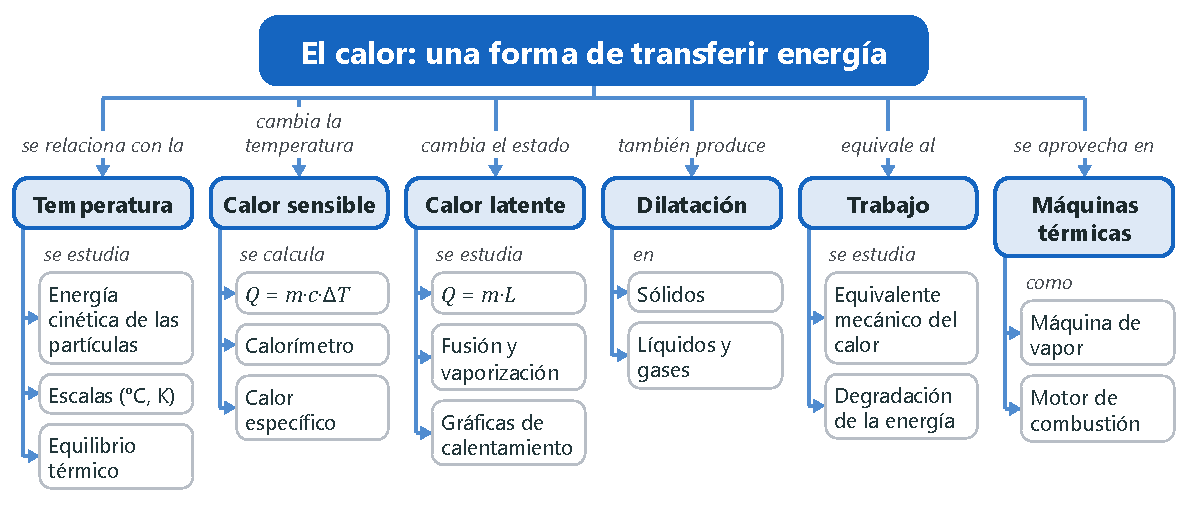
\includegraphics[width=\textwidth]{images/mapas_conceptuales/mapa_UD12}
\end{figure}

%========================================================================================
%\section*{Para empezar: el Sol, una fuente de energía renovable}
%\addcontentsline{toc}{section}{Para empezar: el Sol, una fuente de energía renovable}
%========================================================================================
%
%Casi toda la energía que mueve la «maquinaria» de la Tierra procede del Sol. Su radiación calienta la atmósfera, los océanos y los continentes; produce los vientos; evapora el agua y pone en marcha su ciclo; permite que las plantas realicen la fotosíntesis y, hace millones de años, dio lugar a los combustibles fósiles que hoy usamos en industrias, transportes y hogares.
%
%La humanidad ha aprovechado la energía solar desde siempre, y hoy lo hace de dos formas principales: las \textbf{células fotovoltaicas} transforman la luz del Sol en energía eléctrica, y los \textbf{colectores solares térmicos} la transforman en energía térmica para calentar agua o edificios. La energía solar es \textbf{renovable}, porque se regenera de forma natural, y prácticamente \textbf{inagotable} a escala humana: el Sol seguirá brillando miles de millones de años.
%
%Garantizar a todo el mundo el acceso a una energía asequible, fiable y moderna es el objetivo del \textbf{ODS 7} (\emph{Energía asequible y no contaminante}). Sus metas son aumentar la proporción de energías renovables, duplicar la mejora de la eficiencia energética y fomentar la investigación y la inversión en energías limpias.
%
%En la unidad anterior vimos que la energía se transfiere entre los cuerpos mediante el \textbf{trabajo}. En esta estudiaremos la otra forma de transferir energía, el \textbf{calor}: qué efectos produce (cambios de temperatura, cambios de estado, dilatación), cómo se relaciona con el trabajo y cómo las máquinas térmicas transforman la energía térmica en movimiento.
%
%\begin{exercise}
%    ¿Te parece adecuado el título «El Sol, una fuente de energía renovable e inagotable»? Razona tu respuesta.
%    \begin{solu}
%        \textcolor{red}{Sí}: la energía del Sol se renueva continuamente de forma natural y, a escala de la historia humana, no se agota, pues el Sol seguirá emitiendo energía durante miles de millones de años.
%    \end{solu}
%\end{exercise}
%
%\begin{exercise}
%    Explica tres maneras en las que el Sol influye en el funcionamiento de la naturaleza en la Tierra.
%    \begin{solu}
%        Por ejemplo: \textcolor{red}{calienta la atmósfera, los océanos y los continentes}; origina los \textcolor{red}{vientos} (por las diferencias de temperatura entre unas zonas y otras); pone en marcha el \textcolor{red}{ciclo del agua}; permite la \textcolor{red}{fotosíntesis} y, con ella, el crecimiento de las plantas, que son la base de las cadenas alimentarias.
%    \end{solu}
%\end{exercise}
%
%\begin{exercise}
%    ¿Cómo influyó el Sol en el pasado en la energía que usamos hoy?
%    \begin{solu}
%        La energía del Sol, captada por los seres vivos mediante la fotosíntesis hace millones de años, quedó almacenada en sus restos, que se transformaron en los \textcolor{red}{combustibles fósiles} (carbón, petróleo y gas natural).
%    \end{solu}
%\end{exercise}
%
%\begin{exercise}
%    ¿Por qué se dice que la energía solar es renovable? ¿Es lo mismo «renovable» que «no contaminante»?
%    \begin{solu}
%        Es \textcolor{red}{renovable porque se regenera de forma natural} y su uso no la agota. \textcolor{red}{No es lo mismo}: una fuente es renovable si no se agota, y es poco contaminante si su uso no emite sustancias perjudiciales. La energía solar cumple las dos condiciones durante su uso, aunque fabricar los paneles sí tiene un impacto ambiental.
%    \end{solu}
%\end{exercise}
%
%\begin{exercise}
%    ¿Qué transformación de energía se produce en una célula fotovoltaica? ¿Y en un colector solar térmico?
%    \begin{solu}
%        En la célula fotovoltaica, la energía de la luz se transforma en \textcolor{red}{energía eléctrica}. En el colector solar térmico, se transforma en \textcolor{red}{energía térmica} (calienta un fluido, normalmente agua).
%    \end{solu}
%\end{exercise}
%
%\begin{exercise}
%    Debatid en clase cómo puede contribuir la energía solar a lograr el ODS 7.
%    \begin{solu}
%        Respuesta libre. La energía solar aumenta la proporción de energía renovable (meta 7.2), puede llevar electricidad a zonas aisladas sin red eléctrica (meta 7.1) y, una vez instalada, es barata y no emite gases de efecto invernadero.
%    \end{solu}
%\end{exercise}

%========================================================================================
\section{¿Existe otra forma de intercambiar energía? El calor}
%========================================================================================

Cuando una fuerza desplaza un cuerpo, se intercambia energía mediante un \textbf{trabajo}. Pero hay situaciones en las que se transfiere energía sin que ninguna fuerza desplace nada: al poner una cazuela sobre el fuego, al echar un cubito de hielo en un refresco o al calentarnos las manos junto a un radiador. En todos estos casos se intercambia \textbf{energía térmica}, y esta transferencia se mide por el \textbf{calor}. El calor no se puede calcular con el trabajo, sino a partir de las \textbf{variaciones de temperatura} que produce.

\begin{marker}
    \begin{itemize}
        \item El \textbf{trabajo} y el \textbf{calor} son los dos procesos mediante los cuales los cuerpos intercambian energía.
        \item La energía, el trabajo y el calor se miden en la misma unidad del SI: el \textbf{julio} (\unit{\joule}).
    \end{itemize}
\end{marker}

Un cuerpo no «tiene» calor, igual que no «tiene» trabajo: tiene energía. El calor es la energía \emph{en tránsito}, la que pasa de un cuerpo a otro por estar a distinta temperatura.

\subsection{¿Qué relación existe entre la energía cinética de las partículas y la temperatura?}

Según la \textbf{teoría cinético-molecular}, la materia está formada por partículas (átomos, moléculas o iones) que se mueven continuamente y, por tanto, tienen energía cinética. Cuanto mayor es la temperatura de un cuerpo, más deprisa se mueven sus partículas (figura~\ref{fig:particulas_temperatura}).

\begin{figure}[H]
    \centering
    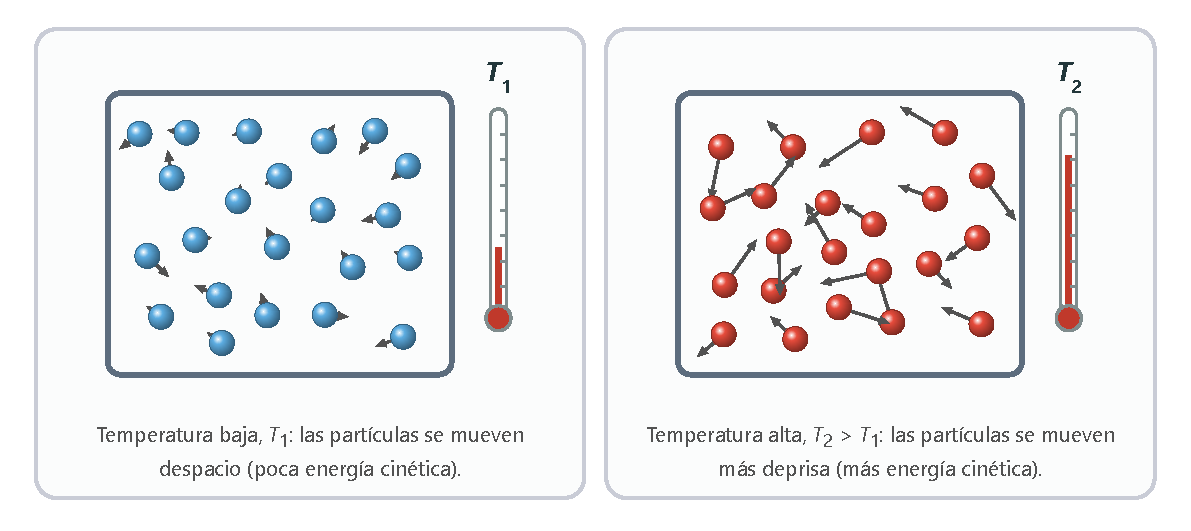
\includegraphics[width=0.9\textwidth]{images/UD12/particulas_temperatura}
    \caption{Al aumentar la temperatura, las partículas se mueven con más velocidad: su energía cinética media es mayor.}
    \label{fig:particulas_temperatura}
\end{figure}

\begin{definition}[Energía térmica y temperatura]
    La \textbf{energía térmica} de un cuerpo está relacionada con la energía cinética de sus partículas. La \textbf{temperatura} es una medida de la \textbf{energía cinética media} de esas partículas.
\end{definition}

Fíjate en la diferencia: un iceberg está más frío que una taza de café, pero, como tiene muchísimas más partículas, su energía térmica total es mucho mayor.

\subsection{Escalas de temperatura}

En la vida diaria medimos la temperatura en grados Celsius (\unit{\degreeCelsius}), pero la unidad del SI es el \textbf{kelvin} (\unit{\kelvin}). La escala Kelvin empieza en el \textbf{cero absoluto} (\qty{-273}{\degreeCelsius}), la temperatura más baja posible, a la que las partículas tendrían la mínima energía. Un kelvin y un grado Celsius tienen el mismo tamaño, así que:
\[ T\,(\unit{\kelvin}) = t\,(\unit{\degreeCelsius}) + 273 \]
Por eso una \textbf{variación} de temperatura vale lo mismo en las dos escalas: si el agua pasa de \qty{20}{\degreeCelsius} a \qty{30}{\degreeCelsius}, ha aumentado \qty{10}{\degreeCelsius} o, lo que es igual, \qty{10}{\kelvin}.

\subsection{¿Qué sucede cuando se ponen en contacto dos cuerpos a diferente temperatura? El equilibrio térmico}

La experiencia nos dice que, si ponemos en contacto dos cuerpos a distinta temperatura, al cabo de un tiempo los dos acaban a la misma temperatura: el café se enfría, el agua del vaso se calienta con la mano\ldots{} Las partículas del cuerpo caliente, al chocar con las del frío, les transfieren parte de su energía cinética (figura~\ref{fig:equilibrio_termico}).

\begin{figure}[H]
    \centering
    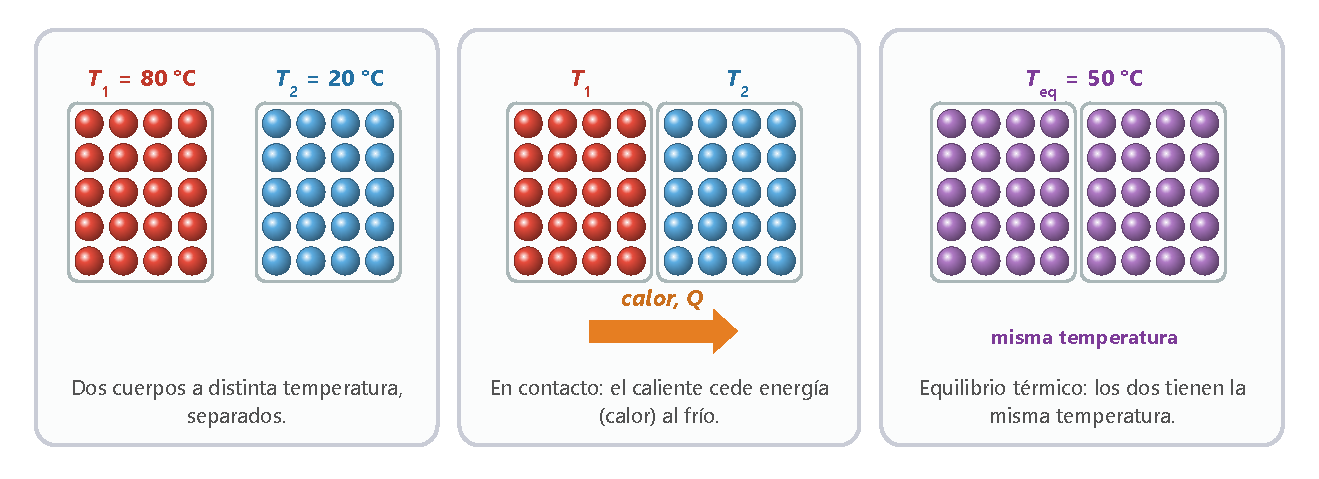
\includegraphics[width=\textwidth]{images/UD12/equilibrio_termico}
    \caption{Dos cuerpos en contacto intercambian energía hasta alcanzar el equilibrio térmico.}
    \label{fig:equilibrio_termico}
\end{figure}

\begin{definition}[Equilibrio térmico y calor]
    \begin{itemize}
        \item Dos cuerpos en contacto que están a la misma temperatura están en \textbf{equilibrio térmico}: ya no intercambian energía.
        \item El \textbf{calor} (\(Q\)) es la energía que se transfiere de un cuerpo a otro debido a su diferencia de temperatura. Pasa siempre, de forma espontánea, \textbf{del cuerpo de mayor temperatura al de menor temperatura}.
    \end{itemize}
\end{definition}

\begin{exercise}
    Razona si son verdaderas o falsas estas afirmaciones:
    \begin{enumerate}[label=\alph*)]
        \item Cuando baja la temperatura, las partículas de la materia se mueven más deprisa.
        \item Si dos cuerpos están a la misma temperatura, la energía cinética media de sus partículas es la misma.
        \item La energía térmica está relacionada con la energía cinética de las partículas del cuerpo.
        \item La energía, el calor y la temperatura se miden en las mismas unidades.
        \item La energía que pasa de un cuerpo a otro de menor temperatura se llama trabajo.
    \end{enumerate}
    \begin{solu}
        a) \textcolor{red}{Falso}: si baja la temperatura, las partículas se mueven más despacio. b) \textcolor{red}{Verdadero}: la temperatura mide la energía cinética media de las partículas. c) \textcolor{red}{Verdadero}. d) \textcolor{red}{Falso}: la energía y el calor se miden en julios, pero la temperatura se mide en \unit{\degreeCelsius} o en \unit{\kelvin}. e) \textcolor{red}{Falso}: se llama calor.
    \end{solu}
\end{exercise}

\begin{exercise}
    Expresa en kelvin estas temperaturas: \qty{25}{\degreeCelsius}, \qty{-18}{\degreeCelsius} y \qty{100}{\degreeCelsius}. Expresa en grados Celsius \qty{0}{\kelvin} y \qty{310}{\kelvin}.
    \begin{solu}
        \(T = t + 273\): \qty{25}{\degreeCelsius} \(\rightarrow\) \textcolor{red}{\qty{298}{\kelvin}}; \qty{-18}{\degreeCelsius} \(\rightarrow\) \textcolor{red}{\qty{255}{\kelvin}}; \qty{100}{\degreeCelsius} \(\rightarrow\) \textcolor{red}{\qty{373}{\kelvin}}. \(t = T - 273\): \qty{0}{\kelvin} \(\rightarrow\) \textcolor{red}{\qty{-273}{\degreeCelsius}}; \qty{310}{\kelvin} \(\rightarrow\) \textcolor{red}{\qty{37}{\degreeCelsius}} (la temperatura del cuerpo humano).
    \end{solu}
\end{exercise}

\subsection*{Actividades de consolidación: el calor}

\begin{exercise}
    Razona si estas afirmaciones son verdaderas o falsas:
    \begin{enumerate}[label=\alph*)]
        \item Entre dos cuerpos en equilibrio térmico no se transfiere calor.
        \item El calor pasa de un cuerpo a otro que está a mayor temperatura.
        \item Dos cuerpos en equilibrio térmico pueden estar a distinta temperatura.
        \item La energía es la forma de intercambiar trabajo y calor.
    \end{enumerate}
    \begin{solu}
        a) \textcolor{red}{Verdadero}. b) \textcolor{red}{Falso}: pasa del cuerpo de mayor temperatura al de menor temperatura. c) \textcolor{red}{Falso}: si están en equilibrio térmico, tienen la misma temperatura. d) \textcolor{red}{Falso}: es al revés; el trabajo y el calor son las formas de intercambiar energía.
    \end{solu}
\end{exercise}

\begin{exercise}
    Ponemos en contacto dos cuerpos a distinta temperatura.
    \begin{enumerate}[label=\alph*)]
        \item ¿Cuándo diremos que han alcanzado el equilibrio térmico?
        \item ¿Qué hay que hacer para que lo alcancen?
        \item ¿Cuál de los dos cede calor al otro?
    \end{enumerate}
    \begin{solu}
        a) Cuando los dos tengan la \textcolor{red}{misma temperatura}. b) Basta con \textcolor{red}{mantenerlos en contacto el tiempo suficiente}. c) El que está a \textcolor{red}{mayor temperatura} cede calor al que está a menor temperatura.
    \end{solu}
\end{exercise}

\begin{exercise}
    ¿En qué sentido se transfiere el calor entre dos cuerpos a diferente temperatura hasta que se alcanza el equilibrio térmico? ¿Puede ocurrir espontáneamente al revés?
    \begin{solu}
        Se transfiere \textcolor{red}{desde el cuerpo de mayor temperatura hacia el de menor temperatura}. \textcolor{red}{No} puede ocurrir al revés de forma espontánea: para sacar calor de un cuerpo frío y llevarlo a uno caliente (como hace un frigorífico) hay que aportar trabajo.
    \end{solu}
\end{exercise}

\begin{exercise}
    En 1798, Benjamin Thompson (conde de Rumford) dirigía la fabricación de cañones en el arsenal de Múnich. Le sorprendió lo mucho que se calentaban, en muy poco tiempo, las piezas de latón al taladrarlas, y todavía más las virutas que saltaban. Tanto, que con ese calor llegó a hacer hervir agua.
    \begin{enumerate}[label=\alph*)]
        \item ¿Qué transformación de energía observó Thompson?
        \item Busca información sobre Thompson y sobre la teoría del calor que se aceptaba en su época (el «calórico»). ¿Por qué fue importante su observación?
    \end{enumerate}
    \begin{solu}
        a) La transformación de \textcolor{red}{energía mecánica} (el trabajo del taladro contra el rozamiento) \textcolor{red}{en energía térmica}.
        b) Respuesta libre. Thompson nació en Norteamérica, luchó en el bando británico en la guerra de independencia de EE.~UU. y después trabajó para el gobierno de Baviera, donde reorganizó el ejército. En su época se pensaba que el calor era un fluido invisible, el \emph{calórico}, que pasaba de unos cuerpos a otros. Thompson se dio cuenta de que el taladro podía producir calor \textcolor{red}{sin límite} mientras siguiera trabajando, algo imposible si el calor fuera una sustancia almacenada en el metal. Su observación apuntaba a que \textcolor{red}{el calor está relacionado con el movimiento}, idea que Joule confirmó medio siglo después.
    \end{solu}
\end{exercise}

\begin{exercise}
    Explica la diferencia entre temperatura, energía térmica y calor usando este ejemplo: una piscina a \qty{25}{\degreeCelsius} y una taza de café a \qty{70}{\degreeCelsius}.
    \begin{solu}
        La \textcolor{red}{temperatura} del café es mayor: sus partículas tienen más energía cinética media. Sin embargo, la piscina tiene \textcolor{red}{más energía térmica}, porque tiene muchísimas más partículas. Si echamos el café en la piscina, se transferirá \textcolor{red}{calor} del café (mayor temperatura) al agua de la piscina, aunque esta tenga más energía térmica.
    \end{solu}
\end{exercise}

%========================================================================================
\section{Cantidad de calor y variación de temperatura}
%========================================================================================

¿Qué relación hay entre el calor que recibe un cuerpo y lo que sube su temperatura? Hagamos dos experiencias con un mismo hornillo, calentando siempre durante el mismo tiempo, de modo que todos los recipientes reciben la misma energía (figura~\ref{fig:calentamiento_experiencias}):
\begin{enumerate}[label=\numberballblue]
    \item Calentamos dos vasos con distinta cantidad de agua (\qty{400}{\gram} y \qty{200}{\gram}), inicialmente a la misma temperatura. El vaso con menos agua acaba más caliente.
    \item Calentamos la misma masa (\qty{400}{\gram}) de agua y de glicerina. La glicerina se calienta más que el agua.
\end{enumerate}

\begin{figure}[H]
    \centering
    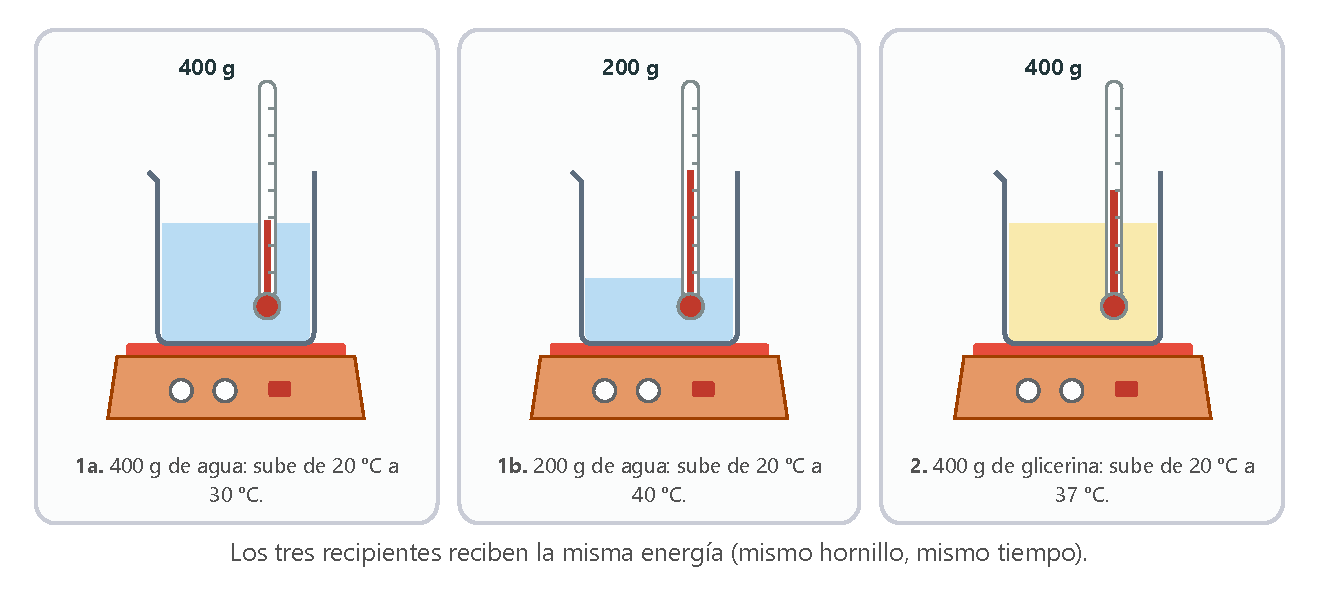
\includegraphics[width=\textwidth]{images/UD12/calentamiento_experiencias}
    \caption{Con la misma energía, la variación de temperatura depende de la masa y de la sustancia.}
    \label{fig:calentamiento_experiencias}
\end{figure}

De estas experiencias se deduce que:
\begin{itemize}
    \item La variación de temperatura depende de la \textbf{masa} del cuerpo: con la misma energía, cuanto más masa, menos sube la temperatura.
    \item La variación de temperatura depende de la \textbf{sustancia}.
    \item La energía transferida es \textbf{proporcional a la variación de temperatura}.
\end{itemize}

Todo ello se resume en una sola expresión:
\begin{equation*}
    \boxed{Q = m \cdot c \cdot (T_2 - T_1) = m \cdot c \cdot \Delta T}
\end{equation*}
donde \(Q\) es el calor transferido (\unit{\joule}); \(m\), la masa (\unit{\kg}); \(T_1\) y \(T_2\), las temperaturas inicial y final (\unit{\degreeCelsius} o \unit{\kelvin}), y \(c\), la \textbf{capacidad calorífica específica} o \textbf{calor específico} de la sustancia. Si el cuerpo se calienta, \(T_2 > T_1\) y \(Q\) es positivo (el cuerpo \emph{absorbe} calor); si se enfría, \(Q\) es negativo (el cuerpo \emph{cede} calor).

\begin{definition}[Capacidad calorífica específica]
    La \textbf{capacidad calorífica específica} (o calor específico), \(c\), de una sustancia es la energía que hay que transferir a \qty{1}{\kg} de esa sustancia para que su temperatura aumente \qty{1}{\degreeCelsius}. Se mide en \unit{\cunit} o, lo que es lo mismo, en \unit{\joule\per\kg\per\kelvin}.
\end{definition}

\begin{center}
    % --- tabla antigua ---
    % \begin{tblr}{colspec={lr}, hlines, vlines, row{1}={bg=ocre!85, fg=white, font=\bfseries}, column{2}={font=\small}}
        % Sustancia & \(c\) (\unit{\cunit}) \\
        % Aluminio & 910 \\
        % Cobre & 386 \\
        % Hierro & 447 \\
        % Plomo & 130 \\
        % Mercurio & 140 \\
        % Oxígeno & 920 \\
        % Agua líquida & 4180 \\
        % Hielo & 2100 \\
        % Glicerina & 2430 \\
    % \end{tblr}
    % --- tabla nueva ---
    {\small
    \begin{tabular}{@{}lr@{}}
        \toprule
        \textbf{Sustancia} & \textbf{\(c\) (\unit{\cunit})} \\
        \midrule
        Aluminio & 910 \\[3pt]
        Cobre & 386 \\[3pt]
        Hierro & 447 \\[3pt]
        Plomo & 130 \\[3pt]
        Mercurio & 140 \\[3pt]
        Oxígeno & 920 \\[3pt]
        Agua líquida & 4180 \\[3pt]
        Hielo & 2100 \\[3pt]
        Glicerina & 2430 \\
        \bottomrule
    \end{tabular}
    }
\end{center}

\begin{remark}
    El agua tiene una capacidad calorífica específica muy alta: hacen falta \qty{4180}{\joule} para que \qty{1}{\kg} de agua líquida suba \qty{1}{\degreeCelsius}. Por eso tarda mucho en calentarse y en enfriarse, y por eso los mares suavizan el clima de las zonas costeras: en verano se calientan menos que la tierra y en invierno se enfrían menos.
\end{remark}

En algunos textos antiguos y en la información nutricional se usa todavía la \textbf{caloría} (\unit{\calorie}), que es el calor necesario para que \qty{1}{\gram} de agua suba \qty{1}{\degreeCelsius}: \(\qty{1}{\calorie} = \qty{4.18}{\joule}\). Las «calorías» de los alimentos son en realidad kilocalorías (\qty{1}{\kilo\calorie} = \qty{4180}{\joule}).

\begin{example}
    Calcula la energía térmica que hay que comunicar a \qty{400}{\gram} de plomo para que su temperatura pase de \qty{15}{\degreeCelsius} a \qty{75}{\degreeCelsius}. Dato: \(c_{\text{Pb}} = \qty{130}{\cunit}\).
    \[ Q = m \cdot c_{\text{Pb}} \cdot (T_2 - T_1) = \num{0.400} \cdot 130 \cdot (75 - 15) = \textcolor{red}{\qty{3120}{\joule}} \]
\end{example}

\begin{exercise}
    Comprueba que la ecuación \(Q = m \cdot c \cdot (T_2 - T_1)\) es homogénea, es decir, que sus dos miembros tienen las mismas dimensiones. (Usa \(\Theta\) para la dimensión de la temperatura.)
    \begin{solu}
        El calor es una energía: \([Q] = \mathrm{M \cdot L^2 \cdot T^{-2}}\). Como \(c = \dfrac{Q}{m \cdot \Delta T}\), sus dimensiones son \([c] = \mathrm{L^2 \cdot T^{-2}} \cdot \Theta^{-1}\). Entonces:
        \[ [m] \cdot [c] \cdot [\Delta T] = \mathrm{M} \cdot \mathrm{L^2 \cdot T^{-2}} \cdot \Theta^{-1} \cdot \Theta = \textcolor{red}{\mathrm{M \cdot L^2 \cdot T^{-2}}} \]
        Los dos miembros tienen las dimensiones de una energía: la ecuación es \textcolor{red}{homogénea}.
    \end{solu}
\end{exercise}

\begin{exercise}
    ¿Qué energía térmica hay que comunicar a \qty{300}{\gram} de aluminio para calentarlos de \qty{20}{\degreeCelsius} a \qty{70}{\degreeCelsius}? Dato: \(c_{\text{Al}} = \qty{910}{\cunit}\).
    \begin{solu}
        \(Q = m \cdot c \cdot \Delta T = \num{0.300} \cdot 910 \cdot (70 - 20) = \textcolor{red}{\qty{13650}{\joule}}\).
    \end{solu}
\end{exercise}

\subsection{¿Cómo se utiliza un calorímetro?}

Un \textbf{calorímetro} es un recipiente construido para que la energía térmica apenas pueda entrar ni salir a través de sus paredes. Tiene paredes dobles, separadas por una cámara aislante, y una tapa con orificios por los que se introducen un \textbf{termómetro} y un \textbf{agitador} (figura~\ref{fig:calorimetro}). Se usa para aislar las sustancias del ambiente y estudiar los intercambios de energía que se producen entre ellas.

\begin{figure}[H]
    \centering
    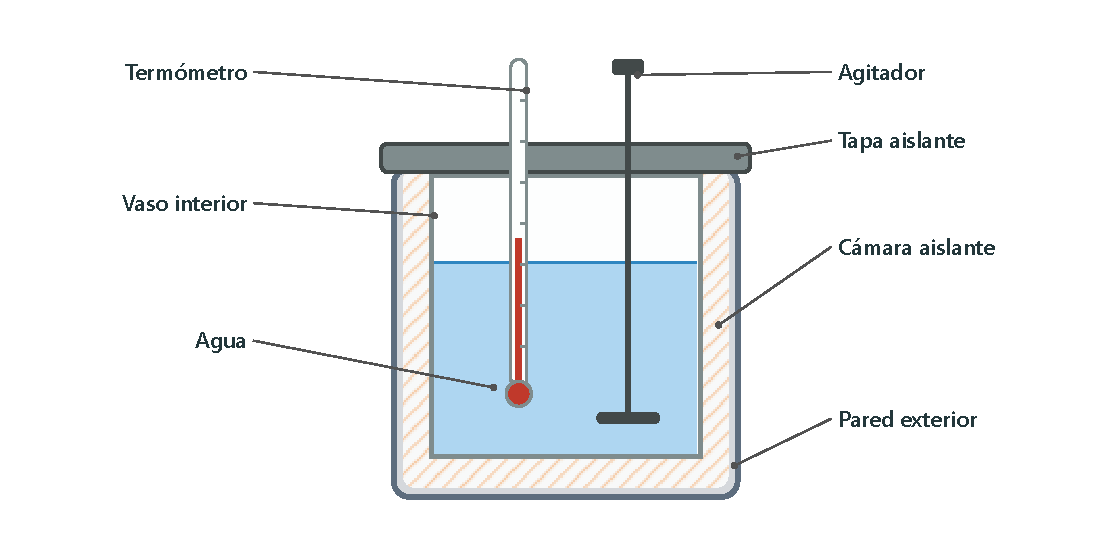
\includegraphics[width=0.8\textwidth]{images/UD12/calorimetro}
    \caption{Esquema de un calorímetro.}
    \label{fig:calorimetro}
\end{figure}

Supongamos que en un calorímetro con una masa \(m_2\) de agua a la temperatura \(T_2\) introducimos un cuerpo de masa \(m_1\) a mayor temperatura, \(T_1\). Al poco tiempo, todo alcanza el equilibrio térmico a la temperatura \(T_{\text{eq}}\), que está entre \(T_2\) y \(T_1\) (figura~\ref{fig:balance_calorimetro}).

\begin{figure}[H]
    \centering
    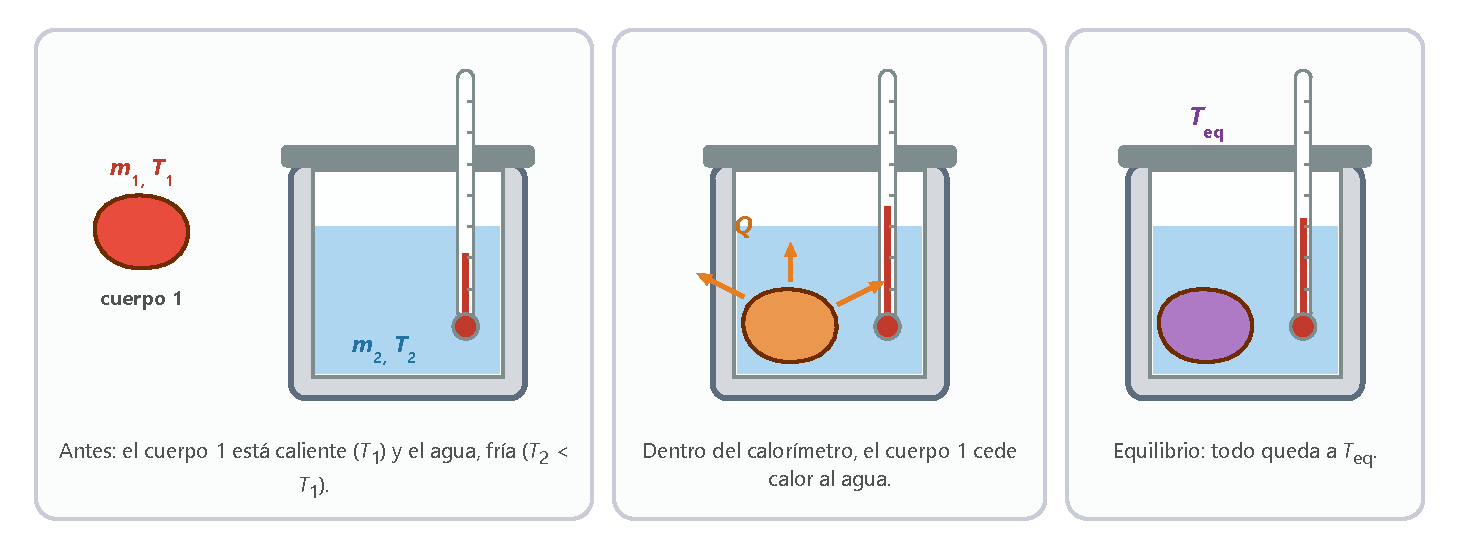
\includegraphics[width=\textwidth]{images/UD12/balance_calorimetro}
    \caption{El cuerpo caliente cede energía al agua hasta que ambos alcanzan el equilibrio térmico.}
    \label{fig:balance_calorimetro}
\end{figure}

\begin{itemize}
    \item Energía cedida por el cuerpo 1, que se enfría: \(Q_1 = m_1 \cdot c_1 \cdot (T_1 - T_{\text{eq}})\).
    \item Energía absorbida por el agua, que se calienta: \(Q_2 = m_2 \cdot c_2 \cdot (T_{\text{eq}} - T_2)\).
\end{itemize}

Como no se escapa energía del calorímetro, toda la energía que cede uno la absorbe el otro:

\begin{definition}[Balance de energía en un calorímetro]
    \[ \text{energía cedida por el cuerpo caliente} = \text{energía absorbida por el cuerpo frío} \]
    \[ \boxed{m_1 \cdot c_1 \cdot (T_1 - T_{\text{eq}}) = m_2 \cdot c_2 \cdot (T_{\text{eq}} - T_2)} \]
\end{definition}

\begin{example}
    Se mezclan \qty{0.6}{\kg} de agua a \qty{80}{\degreeCelsius} con \qty{0.9}{\kg} de agua a \qty{20}{\degreeCelsius}. ¿Qué temperatura tendrá la mezcla en el equilibrio térmico? Dato: \(c_{\text{agua}} = \qty{4180}{\cunit}\).

    El agua caliente cede energía y la fría la absorbe:
    \[ Q_{\text{cedido}} = \num{0.6} \cdot 4180 \cdot (80 - T_{\text{eq}}) \qquad Q_{\text{absorbido}} = \num{0.9} \cdot 4180 \cdot (T_{\text{eq}} - 20) \]
    Igualamos ambas energías; el factor \(c_{\text{agua}}\) aparece en los dos miembros y se simplifica:
    \[ \num{0.6} \cdot (80 - T_{\text{eq}}) = \num{0.9} \cdot (T_{\text{eq}} - 20) \Rightarrow 48 - \num{0.6}\,T_{\text{eq}} = \num{0.9}\,T_{\text{eq}} - 18 \]
    \[ 66 = \num{1.5}\,T_{\text{eq}} \Rightarrow T_{\text{eq}} = \frac{66}{\num{1.5}} = \textcolor{red}{\qty{44}{\degreeCelsius}} \]
    La temperatura queda más cerca de la del agua fría, porque hay más cantidad de ella.
\end{example}

\begin{exercise}
    Se mezclan \qty{3}{\liter} de agua a \qty{20}{\degreeCelsius} con \qty{1}{\liter} de agua a \qty{100}{\degreeCelsius}. ¿Cuál será la temperatura de la mezcla en el equilibrio térmico? (Un litro de agua tiene una masa de \qty{1}{\kg}.)
    \begin{solu}
        \textcolor{blue}{Balance: \(m_1 \cdot c \cdot (T_1 - T_{\text{eq}}) = m_2 \cdot c \cdot (T_{\text{eq}} - T_2)\); como es la misma sustancia, \(c\) se simplifica:}
        \[ 1 \cdot (100 - T_{\text{eq}}) = 3 \cdot (T_{\text{eq}} - 20) \Rightarrow 160 = 4\,T_{\text{eq}} \Rightarrow T_{\text{eq}} = \textcolor{red}{\qty{40}{\degreeCelsius}} \]
    \end{solu}
\end{exercise}

\begin{exercise}
    Queremos enfriar \qty{3}{\kg} de agua a \qty{60}{\degreeCelsius} añadiendo agua a \qty{15}{\degreeCelsius}. ¿Cuánta agua fría hay que añadir para que la mezcla quede a \qty{30}{\degreeCelsius}?
    \begin{solu}
        \textcolor{blue}{Energía cedida por el agua caliente:} \(Q = 3 \cdot 4180 \cdot (60 - 30) = \qty{376200}{\joule}\).

        \textcolor{blue}{La absorbe el agua fría:} \(\num{376200} = m \cdot 4180 \cdot (30 - 15) \Rightarrow m = \dfrac{\num{376200}}{\num{62700}} = \textcolor{red}{\qty{6}{\kg}}\) de agua (6 litros).
    \end{solu}
\end{exercise}

\subsection{Determinación de la capacidad calorífica específica}

Para medir el calor específico de un sólido, lo calentamos hasta una temperatura conocida y lo introducimos en un calorímetro con agua. Midiendo las masas y las temperaturas, el balance de energía nos permite despejar la única incógnita, \(c\):
\[ \text{energía cedida por el sólido} = \text{energía absorbida por el agua} \]

\begin{example}
    Un calorímetro contiene \qty{0.500}{\kg} de agua a \qty{20.0}{\degreeCelsius}. Se introduce un bloque de plomo de \qty{0.200}{\kg} a \qty{95.0}{\degreeCelsius} y, en el equilibrio térmico, el termómetro marca \qty{20.9}{\degreeCelsius}. Calcula la capacidad calorífica específica del plomo.

    Energía absorbida por el agua, que sube \qty{0.9}{\degreeCelsius}:
    \[ Q = m_{\text{agua}} \cdot c_{\text{agua}} \cdot (T_{\text{eq}} - T_{\text{agua}}) = \num{0.500} \cdot 4180 \cdot (\num{20.9} - \num{20.0}) = \qty{1881}{\joule} \]
    Energía cedida por el plomo, que baja de \qty{95.0}{\degreeCelsius} a \qty{20.9}{\degreeCelsius}:
    \[ Q = m_{\text{Pb}} \cdot c_{\text{Pb}} \cdot (T_{\text{Pb}} - T_{\text{eq}}) = \num{0.200} \cdot c_{\text{Pb}} \cdot \num{74.1} = \num{14.82} \cdot c_{\text{Pb}} \]
    Igualamos ambas energías y despejamos:
    \[ c_{\text{Pb}} = \frac{1881}{\num{14.82}} = \textcolor{red}{\qty{127}{\cunit}} \]
    El valor de la tabla es \qty{130}{\cunit}. La pequeña diferencia se debe a los errores de medida (el termómetro aprecia décimas) y a que una parte de la energía se emplea en calentar el propio calorímetro o se pierde al trasladar el bloque.
\end{example}

\begin{exercise}
    En un calorímetro con \qty{1.5}{\liter} de agua a \qty{18}{\degreeCelsius} se introducen \qty{250}{\gram} de un metal a \qty{200}{\degreeCelsius}. Si la temperatura de equilibrio es \qty{24.4}{\degreeCelsius}, ¿cuál es el calor específico del metal? ¿De qué metal puede tratarse?
    \begin{solu}
        \textcolor{blue}{Energía absorbida por el agua:} \(Q = \num{1.5} \cdot 4180 \cdot (\num{24.4} - 18) = \qty{40128}{\joule}\).

        \textcolor{blue}{Energía cedida por el metal:} \(Q = \num{0.250} \cdot c \cdot (200 - \num{24.4}) = \num{43.9} \cdot c\).

        \(c = \dfrac{\num{40128}}{\num{43.9}} \approx \textcolor{red}{\qty{914}{\cunit}}\). Según la tabla, probablemente es \textcolor{red}{aluminio} (\qty{910}{\cunit}).
    \end{solu}
\end{exercise}

\begin{exercise}
    Se introducen \qty{400}{\gram} de una sustancia a \qty{80}{\degreeCelsius} en un calorímetro con \qty{1.5}{\kg} de agua a \qty{15}{\degreeCelsius}. En el equilibrio, el termómetro marca \qty{19}{\degreeCelsius}. Calcula la capacidad calorífica específica de la sustancia.
    \begin{solu}
        \textcolor{blue}{La sustancia se enfría de \qty{80}{\degreeCelsius} a \qty{19}{\degreeCelsius} y el agua se calienta de \qty{15}{\degreeCelsius} a \qty{19}{\degreeCelsius}:}
        \[ \num{0.4} \cdot c \cdot (80 - 19) = \num{1.5} \cdot 4180 \cdot (19 - 15) \Rightarrow \num{24.4} \cdot c = \num{25080} \]
        \[ c = \textcolor{red}{\qty{1028}{\cunit}} \]
    \end{solu}
\end{exercise}

\begin{exercise}
    Un calorímetro contiene \qty{600}{\gram} de agua a \qty{22}{\degreeCelsius}. Se introduce un bloque de cobre de \qty{200}{\gram} a \qty{90}{\degreeCelsius}. Calcula la temperatura de equilibrio. Dato: \(c_{\text{Cu}} = \qty{386}{\cunit}\).
    \begin{solu}
        \textcolor{blue}{Energía absorbida por el agua:} \(\num{0.600} \cdot 4180 \cdot (T_{\text{eq}} - 22) = 2508\,T_{\text{eq}} - \num{55176}\).

        \textcolor{blue}{Energía cedida por el cobre:} \(\num{0.200} \cdot 386 \cdot (90 - T_{\text{eq}}) = 6948 - \num{77.2}\,T_{\text{eq}}\).

        \textcolor{blue}{Igualamos:} \(\num{2585.2}\,T_{\text{eq}} = \num{62124} \Rightarrow T_{\text{eq}} = \textcolor{red}{\qty{24.0}{\degreeCelsius}}\).
    \end{solu}
\end{exercise}

\subsection*{Actividades de consolidación: cantidad de calor y variación de temperatura}

\begin{exercise}
    Copia y completa en tu cuaderno: «La capacidad calorífica específica del hierro es \qty{447}{\cunit}; esto significa que, para que \qty{1}{\kg} de hierro aumente su temperatura \qty{1}{\degreeCelsius}, hay que transferirle \ldots{} J».
    \begin{solu}
        \ldots{} hay que transferirle \textcolor{red}{\qty{447}{\joule}}.
    \end{solu}
\end{exercise}

\begin{exercise}
    ¿Qué energía térmica hay que comunicar a \qty{750}{\gram} de aluminio para elevar su temperatura de \qty{15}{\degreeCelsius} a \qty{75}{\degreeCelsius}? Dato: \(c_{\text{Al}} = \qty{910}{\cunit}\).
    \begin{solu}
        \(Q = \num{0.750} \cdot 910 \cdot (75 - 15) = \textcolor{red}{\qty{40950}{\joule}}\).
    \end{solu}
\end{exercise}

\begin{exercise}
    Se mezclan \qty{0.6}{\kg} de agua a \qty{75}{\degreeCelsius} con \qty{0.4}{\kg} de agua a \qty{25}{\degreeCelsius}. ¿Cuál será la temperatura de la mezcla en el equilibrio térmico?
    \begin{solu}
        \(\num{0.6} \cdot (75 - T_{\text{eq}}) = \num{0.4} \cdot (T_{\text{eq}} - 25) \Rightarrow 45 + 10 = T_{\text{eq}} \Rightarrow T_{\text{eq}} = \textcolor{red}{\qty{55}{\degreeCelsius}}\).
    \end{solu}
\end{exercise}

\begin{exercise}
    ¿Qué energía térmica se necesita para calentar \qty{250}{\gram} de agua desde \qty{10}{\degreeCelsius} hasta \qty{60}{\degreeCelsius}?
    \begin{solu}
        \(Q = \num{0.250} \cdot 4180 \cdot 50 = \textcolor{red}{\qty{52250}{\joule}}\).
    \end{solu}
\end{exercise}

\begin{exercise}
    ¿Qué energía se necesita para elevar \qty{25}{\degreeCelsius} la temperatura de \qty{300}{\gram} de cobre? Dato: \(c_{\text{Cu}} = \qty{386}{\cunit}\).
    \begin{solu}
        \(Q = \num{0.300} \cdot 386 \cdot 25 = \textcolor{red}{\qty{2895}{\joule}}\).
    \end{solu}
\end{exercise}

\begin{exercise}
    ¿Cuánto aumenta la temperatura de \qty{1}{\kg} de cobre si le comunicamos \qty{772}{\joule}?
    \begin{solu}
        \(\Delta T = \dfrac{Q}{m \cdot c} = \dfrac{772}{1 \cdot 386} = \textcolor{red}{\qty{2}{\degreeCelsius}}\).
    \end{solu}
\end{exercise}

\begin{exercise}
    ¿Qué energía térmica hay que transferir a \qty{3}{\kg} de plomo para que su temperatura suba \qty{20}{\degreeCelsius}? Dato: \(c_{\text{Pb}} = \qty{130}{\cunit}\).
    \begin{solu}
        \(Q = 3 \cdot 130 \cdot 20 = \textcolor{red}{\qty{7800}{\joule}}\).
    \end{solu}
\end{exercise}

\begin{exercise}
    ¿Qué energía se necesita para calentar una barra de hierro de \qty{800}{\gram} desde \qty{20}{\degreeCelsius} hasta \qty{120}{\degreeCelsius}? Dato: \(c_{\text{Fe}} = \qty{447}{\cunit}\).
    \begin{solu}
        \(Q = \num{0.800} \cdot 447 \cdot (120 - 20) = \textcolor{red}{\qty{35760}{\joule}}\).
    \end{solu}
\end{exercise}

\begin{exercise}
    Un cuerpo de \qty{4}{\kg} tiene una capacidad calorífica específica de \qty{394}{\cunit}. ¿Cuánta energía hay que suministrarle para calentarlo de \qty{10}{\degreeCelsius} a \qty{40}{\degreeCelsius}? ¿Y si fuera de agua?
    \begin{solu}
        \(Q = 4 \cdot 394 \cdot 30 = \textcolor{red}{\qty{47280}{\joule}}\). Si fuera agua: \(Q = 4 \cdot 4180 \cdot 30 = \textcolor{red}{\qty{501600}{\joule}}\), más de diez veces más.
    \end{solu}
\end{exercise}

\begin{exercise}
    Responde a estas preguntas:
    \begin{enumerate}[label=\alph*)]
        \item ¿Qué es la capacidad calorífica específica? ¿En qué unidades se mide?
        \item Busca dos sustancias, que no estén en la tabla de la unidad, con una capacidad calorífica específica alta.
        \item Busca dos sustancias, que no estén en la tabla, con una capacidad calorífica específica baja.
    \end{enumerate}
    \begin{solu}
        a) Es la energía que hay que transferir a \qty{1}{\kg} de una sustancia para que su temperatura suba \qty{1}{\degreeCelsius}. Se mide en \textcolor{red}{\unit{\cunit}} (o \unit{\joule\per\kg\per\kelvin}).
        b) Respuesta libre. Por ejemplo, el \textcolor{red}{etanol} (unos \qty{2440}{\cunit}), el \textcolor{red}{aceite de oliva} (unos \qty{2000}{\cunit}) o la \textcolor{red}{madera} (unos \qty{1700}{\cunit}).
        c) Respuesta libre. Los metales tienen calores específicos bajos: por ejemplo, la \textcolor{red}{plata} (unos \qty{235}{\cunit}) o el \textcolor{red}{oro} (unos \qty{129}{\cunit}).
    \end{solu}
\end{exercise}

\begin{exercise}
    Se necesitan \qty{2430}{\joule} para elevar \qty{1}{\degreeCelsius} la temperatura de \qty{1}{\kg} de una sustancia. ¿Cuál es su capacidad calorífica específica? ¿Qué sustancia de la tabla puede ser?
    \begin{solu}
        \(c = \textcolor{red}{\qty{2430}{\cunit}}\); según la tabla, se trata de la \textcolor{red}{glicerina}.
    \end{solu}
\end{exercise}

\begin{exercise}
    Un trozo de metal de \qty{80}{\gram} se calienta a \qty{180}{\degreeCelsius} y se introduce en un calorímetro con \qty{0.4}{\kg} de agua a \qty{18}{\degreeCelsius}. Si la temperatura final de equilibrio es \qty{21}{\degreeCelsius}, calcula la capacidad calorífica específica del metal.
    \begin{solu}
        \textcolor{blue}{Energía absorbida por el agua:} \(Q = \num{0.4} \cdot 4180 \cdot (21 - 18) = \qty{5016}{\joule}\).

        \textcolor{blue}{Energía cedida por el metal:} \(Q = \num{0.080} \cdot c \cdot (180 - 21) = \num{12.72} \cdot c\).

        \(c = \dfrac{5016}{\num{12.72}} = \textcolor{red}{\qty{394}{\cunit}}\) (un valor parecido al del cobre o al del latón).
    \end{solu}
\end{exercise}

\begin{exercise}
    Queremos medir la capacidad calorífica específica de una pieza de cobre con un calorímetro.
    \begin{enumerate}[label=\alph*)]
        \item ¿Para qué sirve un calorímetro?
        \item Dibuja un esquema de un calorímetro y señala sus partes.
        \item ¿Qué instrumento de medida lleva incorporado?
    \end{enumerate}
    \begin{solu}
        a) Sirve para \textcolor{red}{aislar del ambiente} las sustancias y estudiar los intercambios de energía térmica entre ellas, por ejemplo, para medir calores específicos.
        b) Como en la figura~\ref{fig:calorimetro}: \textcolor{red}{pared exterior, cámara aislante, vaso interior con el agua, tapa aislante, termómetro y agitador}.
        c) Un \textcolor{red}{termómetro}.
    \end{solu}
\end{exercise}

\begin{exercise}
    Se calientan \qty{400}{\gram} de cobre a \qty{100}{\degreeCelsius} y se introducen en un calorímetro con \qty{600}{\gram} de agua a \qty{16}{\degreeCelsius}. Al poco tiempo, el termómetro marca \qty{20.8}{\degreeCelsius}.
    \begin{enumerate}[label=\alph*)]
        \item Calcula con estos datos la capacidad calorífica específica del cobre.
        \item Compara el resultado con el de la tabla. ¿A qué puede deberse la diferencia?
    \end{enumerate}
    \begin{solu}
        a) \(\num{0.4} \cdot c_{\text{Cu}} \cdot (100 - \num{20.8}) = \num{0.6} \cdot 4180 \cdot (\num{20.8} - 16) \Rightarrow \num{31.68} \cdot c_{\text{Cu}} = \num{12038.4}\)
        \[ c_{\text{Cu}} = \textcolor{red}{\qty{380}{\cunit}} \]
        b) La tabla da \qty{386}{\cunit}. La diferencia se debe a las \textcolor{red}{pérdidas de energía} (parte del calor calienta el propio calorímetro o escapa al ambiente) y a los \textcolor{red}{errores de medida}.
    \end{solu}
\end{exercise}

\begin{exercise}
    Mezclamos \qty{600}{\gram} de una sustancia a \qty{20}{\degreeCelsius} con \qty{200}{\gram} de la misma sustancia a \qty{80}{\degreeCelsius}. ¿Cuál será la temperatura de la mezcla en el equilibrio térmico?
    \begin{solu}
        \(\num{0.6} \cdot c \cdot (T_{\text{eq}} - 20) = \num{0.2} \cdot c \cdot (80 - T_{\text{eq}}) \Rightarrow \num{0.8}\,T_{\text{eq}} = 28 \Rightarrow T_{\text{eq}} = \textcolor{red}{\qty{35}{\degreeCelsius}}\). No hace falta conocer \(c\), porque se simplifica.
    \end{solu}
\end{exercise}

\begin{exercise}
    Se mezclan \qty{3}{\liter} de agua a \qty{30}{\degreeCelsius} con \qty{2}{\liter} de agua a \qty{90}{\degreeCelsius}. ¿Qué temperatura alcanza la mezcla?
    \begin{solu}
        \(3 \cdot (T_{\text{eq}} - 30) = 2 \cdot (90 - T_{\text{eq}}) \Rightarrow 5\,T_{\text{eq}} = 270 \Rightarrow T_{\text{eq}} = \textcolor{red}{\qty{54}{\degreeCelsius}}\).
    \end{solu}
\end{exercise}

\begin{exercise}
    Un kilogramo de mercurio y un kilogramo de agua reciben la misma energía térmica. ¿Cuál de los dos se calienta más? ¿Por qué?
    \begin{solu}
        Se calienta más el \textcolor{red}{mercurio}, porque su capacidad calorífica específica (\qty{140}{\cunit}) es mucho menor que la del agua (\qty{4180}{\cunit}): con la misma energía, su temperatura sube unas 30 veces más.
    \end{solu}
\end{exercise}

\begin{exercise}
    Una pieza de hierro de \qty{200}{\gram} a \qty{90}{\degreeCelsius} se introduce en un termo con \qty{400}{\gram} de agua a \qty{18}{\degreeCelsius}. Describe lo que ocurre y calcula la temperatura final. Dato: \(c_{\text{Fe}} = \qty{447}{\cunit}\).
    \begin{solu}
        Se transfiere energía del cuerpo de mayor temperatura (el hierro) al de menor temperatura (el agua) hasta que ambos alcanzan la misma temperatura.
        \[ \num{0.2} \cdot 447 \cdot (90 - T_{\text{eq}}) = \num{0.4} \cdot 4180 \cdot (T_{\text{eq}} - 18) \]
        \[ 8046 - \num{89.4}\,T_{\text{eq}} = 1672\,T_{\text{eq}} - \num{30096} \Rightarrow T_{\text{eq}} = \frac{\num{38142}}{\num{1761.4}} = \textcolor{red}{\qty{21.7}{\degreeCelsius}} \]
    \end{solu}
\end{exercise}

\begin{exercise}
    Un hervidor eléctrico calienta \qty{4}{\liter} de agua de \qty{15}{\degreeCelsius} a \qty{85}{\degreeCelsius} en \qty{15}{\minute}. ¿Qué energía térmica proporciona cada minuto? ¿Cuál es su potencia útil?
    \begin{solu}
        \(Q = 4 \cdot 4180 \cdot (85 - 15) = \qty{1170400}{\joule}\). Cada minuto: \(\dfrac{\num{1170400}}{15} \approx \textcolor{red}{\qty{78000}{\joule}}\). Potencia útil: \(P = \dfrac{Q}{t} = \dfrac{\num{1170400}}{900} \approx \textcolor{red}{\qty{1300}{\watt}}\).
    \end{solu}
\end{exercise}

\begin{exercise}
    En un calorímetro se mezcla una masa \(m_1\) de plomo a la temperatura \(T_1\) con una masa \(m_2\) de agua a la temperatura \(T_2\), menor que \(T_1\). Al poco tiempo se alcanza el equilibrio a \(T_{\text{eq}}\). Indica cuáles de estas afirmaciones son falsas y corrígelas:
    \begin{enumerate}[label=\alph*)]
        \item La energía absorbida por el plomo es igual a la energía cedida por el agua.
        \item La temperatura de equilibrio es menor que la temperatura inicial del plomo.
        \item La temperatura de equilibrio es menor que la temperatura inicial del agua.
        \item \(m_1 \cdot c_{\text{Pb}} \cdot (T_1 - T_{\text{eq}}) = m_2 \cdot c_{\text{agua}} \cdot (T_{\text{eq}} - T_2)\).
        \item La energía que el plomo transfiere al agua hace que la temperatura de esta aumente.
    \end{enumerate}
    \begin{solu}
        Son falsas \textcolor{red}{a) y c)}. a) Es al revés: la energía \emph{cedida} por el plomo es igual a la \emph{absorbida} por el agua. c) La temperatura de equilibrio es \emph{mayor} que la temperatura inicial del agua (el agua se calienta). b), d) y e) son verdaderas.
    \end{solu}
\end{exercise}

%========================================================================================
\section[Calor en los cambios de estado]{Cantidad de calor transferida en los cambios de estado}
%========================================================================================

Hasta ahora, cuando un cuerpo recibía o cedía energía térmica, su temperatura cambiaba. Pero hay una excepción importante: \textbf{mientras una sustancia pura cambia de estado, su temperatura permanece constante}, aunque siga recibiendo (o cediendo) energía.

Podemos comprobarlo fundiendo naftalina. Ponemos unas bolitas de naftalina en un tubo de ensayo con un termómetro cuyo bulbo quede cubierto, introducimos el tubo en un vaso con agua y lo calentamos. Cada minuto anotamos la temperatura, mientras agitamos el agua, y representamos la temperatura frente al tiempo.

\subsection{Análisis de una gráfica de calentamiento}

\begin{center}
    \begin{tikzpicture}
        \begin{axis}[grafica, width=8cm, height=5.5cm, xlabel={\(t\) (min)}, ylabel={\(T\) (\unit{\degreeCelsius})}, xmin=0, xmax=13, ymin=72, ymax=86, xtick={0,2,...,12}, ytick={72,74,...,86}, title={\small Calentamiento de la naftalina}]
            \addplot[mark=none] coordinates {(0,74) (6,80) (10,80) (12,84)};
            \node[anchor=south, font=\footnotesize] at (axis cs:8,80.2) {fusión (sólido + líquido)};
            \node[anchor=west, font=\footnotesize] at (axis cs:2.2,75.4) {sólido};
            \node[anchor=east, font=\footnotesize] at (axis cs:10.6,83.6) {líquido};
        \end{axis}
    \end{tikzpicture}
\end{center}

En la gráfica se distinguen tres tramos:
\begin{enumerate}[label=\numberballblue]
    \item Un tramo ascendente: la naftalina sólida se calienta hasta \qty{80}{\degreeCelsius}, su \textbf{temperatura de fusión}.
    \item Un tramo \textbf{horizontal}: mientras se funde, la temperatura no cambia. Se mantiene constante \textbf{durante todo el cambio de estado}, hasta que toda la naftalina es líquida.
    \item Otro tramo ascendente: la naftalina líquida sigue calentándose.
\end{enumerate}

\subsection{El calor latente de cambio de estado}

¿En qué se emplea la energía que recibe la sustancia durante el cambio de estado, si no aumenta su temperatura? Se usa en \textbf{vencer las fuerzas de cohesión} que mantienen unidas las partículas en el sólido (en la fusión) o en el líquido (en la vaporización). La energía cinética media de las partículas no cambia, así que el termómetro no detecta nada; por eso decimos que es un calor «latente» (escondido).

\begin{definition}[Calor latente de cambio de estado]
    El \textbf{calor latente}, \(L\), de un cambio de estado es la energía que hay que transferir a \qty{1}{\kg} de una sustancia pura para que cambie de estado, a una presión determinada y a la temperatura del cambio de estado. Se mide en \unit{\joule\per\kg}. El calor necesario para que cambie de estado una masa \(m\) es:
    \[ \boxed{Q = m \cdot L} \]
\end{definition}

\subsection{Calor latente de fusión y de vaporización}

En la gráfica de calentamiento de una sustancia desde el estado sólido hasta el gaseoso aparecen dos tramos horizontales:
\begin{itemize}
    \item El primero corresponde a la \textbf{fusión} (paso de sólido a líquido). El calor necesario es \(Q = m \cdot L_f\), donde \(L_f\) es el \textbf{calor latente de fusión}. Es igual al calor latente de solidificación, pero en la fusión la sustancia \emph{absorbe} esa energía y en la solidificación la \emph{cede}.
    \item El segundo corresponde a la \textbf{vaporización} (paso de líquido a gas). El calor necesario es \(Q = m \cdot L_v\), donde \(L_v\) es el \textbf{calor latente de vaporización}, igual al de condensación: para vaporizar hay que aportar energía, y al condensarse el vapor la desprende.
\end{itemize}

\begin{center}
    % --- tabla antigua ---
    % \begin{tblr}{colspec={lcccc}, hlines, vlines, row{1}={bg=ocre!85, fg=white, font=\bfseries\small}, cells={font=\small}}
        % Sustancia & \(T_f\) (\unit{\degreeCelsius}) & \(L_f\) (\unit{\joule\per\kg}) & \(T_{eb}\) (\unit{\degreeCelsius}) & \(L_v\) (\unit{\joule\per\kg}) \\
        % Agua & 0 & \num{3.35e5} & 100 & \num{2.2e6} \\
        % Aluminio & 660 & \num{4.0e5} & 2470 & \num{1.05e7} \\
        % Cobre & 1085 & \num{2.05e5} & 2560 & \num{4.8e6} \\
        % Hierro & 1538 & \num{2.75e5} & 2860 & \num{6.3e6} \\
        % Plomo & 327 & \num{2.3e4} & 1750 & \num{8.6e5} \\
        % Mercurio & \num{-39} & \num{1.1e4} & 357 & \num{2.9e5} \\
    % \end{tblr}
    % --- tabla nueva ---
    {\small
    \begin{tabular}{@{}lcccc@{}}
        \toprule
        \textbf{Sustancia} & \textbf{\(T_f\) (\unit{\degreeCelsius})} & \textbf{\(L_f\) (\unit{\joule\per\kg})} & \textbf{\(T_{eb}\) (\unit{\degreeCelsius})} & \textbf{\(L_v\) (\unit{\joule\per\kg})} \\
        \midrule
        Agua & 0 & \num{3.35e5} & 100 & \num{2.2e6} \\[3pt]
        Aluminio & 660 & \num{4.0e5} & 2470 & \num{1.05e7} \\[3pt]
        Cobre & 1085 & \num{2.05e5} & 2560 & \num{4.8e6} \\[3pt]
        Hierro & 1538 & \num{2.75e5} & 2860 & \num{6.3e6} \\[3pt]
        Plomo & 327 & \num{2.3e4} & 1750 & \num{8.6e5} \\[3pt]
        Mercurio & \num{-39} & \num{1.1e4} & 357 & \num{2.9e5} \\
        \bottomrule
    \end{tabular}
    }
\end{center}

Observa que el calor latente de vaporización del agua es casi siete veces mayor que el de fusión: separar por completo las moléculas del líquido cuesta mucha más energía que deshacer la estructura del hielo.

\begin{example}
    Calcula la energía que hay que transferir a \qty{2}{\kg} de hielo a \qty{-10}{\degreeCelsius} para convertirlos en vapor de agua a \qty{100}{\degreeCelsius}. Datos: \(c_{\text{hielo}} = \qty{2100}{\cunit}\); \(c_{\text{agua}} = \qty{4180}{\cunit}\); \(L_f = \qty{3.35e5}{\joule\per\kg}\); \(L_v = \qty{2.2e6}{\joule\per\kg}\).

    \begin{center}
        \begin{tikzpicture}
            \begin{axis}[grafica, width=9cm, height=5.5cm, xlabel={\(t\)}, ylabel={\(T\) (\unit{\degreeCelsius})}, xmin=0, xmax=12, ymin=-20, ymax=120, xtick=\empty, ytick={-10,0,100}, title={\small Calentamiento del agua}]
                \addplot[mark=none] coordinates {(0,-10) (0.6,0) (2.2,0) (4.2,100) (10.2,100) (11,115)};
                \node[anchor=west, font=\scriptsize] at (axis cs:0.5,-12) {tramo 1: hielo};
                \node[anchor=south, font=\scriptsize] at (axis cs:1.4,2) {tramo 2};
                \node[anchor=west, font=\scriptsize] at (axis cs:3.3,45) {tramo 3: líquido};
                \node[anchor=south, font=\scriptsize] at (axis cs:7.2,102) {tramo 4: vaporización};
            \end{axis}
        \end{tikzpicture}
    \end{center}

    Analizamos cada tramo de la gráfica:
    \begin{itemize}
        \item \textbf{Tramo 1}. El hielo se calienta de \qty{-10}{\degreeCelsius} a \qty{0}{\degreeCelsius}:\\ \(Q_1 = m \cdot c_{\text{hielo}} \cdot \Delta T = 2 \cdot 2100 \cdot 10 = \qty{42000}{\joule}\).
        \item \textbf{Tramo 2}. El hielo se funde a \qty{0}{\degreeCelsius} (la temperatura no cambia):\\ \(Q_2 = m \cdot L_f = 2 \cdot \num{3.35e5} = \qty{670000}{\joule}\).
        \item \textbf{Tramo 3}. El agua líquida se calienta de \qty{0}{\degreeCelsius} a \qty{100}{\degreeCelsius}:\\ \(Q_3 = m \cdot c_{\text{agua}} \cdot \Delta T = 2 \cdot 4180 \cdot 100 = \qty{836000}{\joule}\).
        \item \textbf{Tramo 4}. El agua hierve a \qty{100}{\degreeCelsius} hasta convertirse toda en vapor:\\ \(Q_4 = m \cdot L_v = 2 \cdot \num{2.2e6} = \qty{4400000}{\joule}\).
    \end{itemize}
    La energía total es la suma de los cuatro tramos:
    \[ Q_{\text{total}} = Q_1 + Q_2 + Q_3 + Q_4 = \textcolor{red}{\qty{5948000}{\joule} \approx \qty{5.95e6}{\joule}} \]
    Fíjate en que la vaporización (tramo 4) se lleva casi las tres cuartas partes de la energía.
\end{example}

\begin{exercise}
    Quieres averiguar experimentalmente el punto de fusión de una cera, sólida a temperatura ambiente, y obtienes esta gráfica de calentamiento. ¿Cuál es su punto de fusión? ¿Y su punto de solidificación? ¿Qué significa el tramo paralelo al eje de abscisas?
    \begin{center}
        \begin{tikzpicture}
            \begin{axis}[grafica, width=7.5cm, height=5cm, xlabel={\(t\) (min)}, ylabel={\(T\) (\unit{\degreeCelsius})}, xmin=0, xmax=15, ymin=20, ymax=80, xtick={0,2,...,14}, ytick={20,30,...,80}]
                \addplot[mark=none] coordinates {(0,25) (6,55) (10,55) (14,75)};
            \end{axis}
        \end{tikzpicture}
    \end{center}
    \begin{solu}
        El punto de fusión es \textcolor{red}{\qty{55}{\degreeCelsius}}, y el de solidificación es el mismo, \textcolor{red}{\qty{55}{\degreeCelsius}}. El tramo horizontal indica que la \textcolor{red}{temperatura se mantiene constante mientras dura el cambio de estado}: la energía que recibe la cera se emplea en fundirla.
    \end{solu}
\end{exercise}

\begin{exercise}
    Calcula la energía que hay que transferir a \qty{1.5}{\kg} de hielo a \qty{-8}{\degreeCelsius} para calentarlo hasta \qty{100}{\degreeCelsius} y convertir toda el agua en vapor.
    \begin{solu}
        \textcolor{blue}{Tramo 1 (hielo de \qty{-8}{\degreeCelsius} a \qty{0}{\degreeCelsius}):} \(Q_1 = \num{1.5} \cdot 2100 \cdot 8 = \qty{25200}{\joule}\).

        \textcolor{blue}{Tramo 2 (fusión):} \(Q_2 = \num{1.5} \cdot \num{3.35e5} = \qty{502500}{\joule}\).

        \textcolor{blue}{Tramo 3 (agua de \qty{0}{\degreeCelsius} a \qty{100}{\degreeCelsius}):} \(Q_3 = \num{1.5} \cdot 4180 \cdot 100 = \qty{627000}{\joule}\).

        \textcolor{blue}{Tramo 4 (vaporización):} \(Q_4 = \num{1.5} \cdot \num{2.2e6} = \qty{3300000}{\joule}\).

        \(Q_{\text{total}} = \qty{4454700}{\joule} \approx \textcolor{red}{\qty{4.45e6}{\joule}}\).
    \end{solu}
\end{exercise}

\subsection*{Actividades de consolidación: calor en los cambios de estado}

\begin{exercise}
    Para que una sustancia pura pase de sólido a líquido, o de líquido a gas, hay que darle energía; sin embargo, su temperatura no cambia durante el cambio de estado. ¿En qué se emplea esa energía?
    \begin{solu}
        Se emplea en \textcolor{red}{vencer las fuerzas de cohesión} que mantienen unidas las partículas en el sólido (fusión) o en el líquido (vaporización). La energía cinética media de las partículas no aumenta, por eso no sube la temperatura.
    \end{solu}
\end{exercise}

\begin{exercise}
    ¿Pueden tener dos sustancias puras distintas el mismo punto de fusión? ¿Basta con medir el punto de fusión para identificar una sustancia?
    \begin{solu}
        \textcolor{red}{Sí pueden}: el punto de fusión es una propiedad característica, pero hay miles de sustancias y algunas coinciden (o tienen valores muy próximos). Por eso \textcolor{red}{no basta con una sola propiedad}: para identificar una sustancia se miden varias (punto de fusión, punto de ebullición, densidad, calor específico\ldots).
    \end{solu}
\end{exercise}

\begin{exercise}
    Responde:
    \begin{enumerate}[label=\alph*)]
        \item ¿Cómo varía la temperatura de una sustancia pura durante un cambio de estado?
        \item ¿Qué es el calor latente?
        \item ¿En qué unidades se expresa?
    \end{enumerate}
    \begin{solu}
        a) \textcolor{red}{Permanece constante}. b) Es la energía que hay que transferir a \qty{1}{\kg} de una sustancia para que cambie de estado (a la temperatura del cambio de estado). c) En \textcolor{red}{\unit{\joule\per\kg}}.
    \end{solu}
\end{exercise}

\begin{exercise}
    Dibuja la gráfica de calentamiento de una masa de agua que pasa por estas fases: 1) inicialmente es hielo a \qty{-15}{\degreeCelsius}; 2) se calienta hasta \qty{0}{\degreeCelsius}; 3) se funde a \qty{0}{\degreeCelsius}; 4) el agua líquida se calienta hasta \qty{100}{\degreeCelsius}; 5) el agua hierve a \qty{100}{\degreeCelsius} hasta convertirse toda en vapor.
    \begin{solu}
        \begin{center}
            \begin{tikzpicture}
                \begin{axis}[grafica, width=7.5cm, height=5cm, xlabel={\(t\)}, ylabel={\(T\) (\unit{\degreeCelsius})}, xmin=0, xmax=11, ymin=-25, ymax=115, xtick=\empty, ytick={-15,0,100}]
                    \addplot[mark=none] coordinates {(0,-15) (0.8,0) (2.4,0) (4.4,100) (10,100)};
                    \node[anchor=west, font=\scriptsize] at (axis cs:0.6,-18) {hielo};
                    \node[anchor=south, font=\scriptsize] at (axis cs:1.6,2) {fusión};
                    \node[anchor=west, font=\scriptsize] at (axis cs:3.5,45) {líquido};
                    \node[anchor=north, font=\scriptsize] at (axis cs:7.2,97) {vaporización};
                \end{axis}
            \end{tikzpicture}
        \end{center}
        Tiene \textcolor{red}{dos tramos horizontales} (a \qty{0}{\degreeCelsius} y a \qty{100}{\degreeCelsius}); el de la vaporización es mucho más largo, porque \(L_v\) es mucho mayor que \(L_f\).
    \end{solu}
\end{exercise}

\begin{exercise}
    ¿Por qué un refresco se enfría más con un cubito de hielo a \qty{0}{\degreeCelsius} que con la misma masa de agua líquida, también a \qty{0}{\degreeCelsius}?
    \begin{solu}
        Porque el hielo, antes de calentarse, tiene que \textcolor{red}{fundirse}, y para ello absorbe del refresco \(\qty{3.35e5}{\joule}\) por cada kilogramo (el calor latente de fusión), sin cambiar de temperatura. El agua líquida a \qty{0}{\degreeCelsius} no absorbe esa energía extra.
    \end{solu}
\end{exercise}

\begin{exercise}
    ¿Qué calor hace falta para convertir \qty{400}{\gram} de hielo a \qty{0}{\degreeCelsius} en agua líquida a \qty{0}{\degreeCelsius}?
    \begin{solu}
        \(Q = m \cdot L_f = \num{0.400} \cdot \num{3.35e5} = \textcolor{red}{\qty{134000}{\joule}}\).
    \end{solu}
\end{exercise}

\begin{exercise}
    Se calientan \qty{2}{\kg} de hielo a \qty{-15}{\degreeCelsius} hasta que se funden por completo. ¿Qué energía térmica se ha necesitado?
    \begin{solu}
        \(Q_1 = 2 \cdot 2100 \cdot 15 = \qty{63000}{\joule}\) (calentar el hielo hasta \qty{0}{\degreeCelsius}); \(Q_2 = 2 \cdot \num{3.35e5} = \qty{670000}{\joule}\) (fundirlo).
        \(Q = Q_1 + Q_2 = \textcolor{red}{\qty{733000}{\joule}}\).
    \end{solu}
\end{exercise}

\begin{exercise}
    Calcula la energía que hay que transferir a \qty{300}{\gram} de hielo a \qty{-20}{\degreeCelsius} para calentarlo hasta \qty{100}{\degreeCelsius} y vaporizar toda el agua.
    \begin{solu}
        \textcolor{blue}{Tramo 1:} \(Q_1 = \num{0.3} \cdot 2100 \cdot 20 = \qty{12600}{\joule}\). \textcolor{blue}{Tramo 2:} \(Q_2 = \num{0.3} \cdot \num{3.35e5} = \qty{100500}{\joule}\).
        \textcolor{blue}{Tramo 3:} \(Q_3 = \num{0.3} \cdot 4180 \cdot 100 = \qty{125400}{\joule}\). \textcolor{blue}{Tramo 4:} \(Q_4 = \num{0.3} \cdot \num{2.2e6} = \qty{660000}{\joule}\).

        \(Q_{\text{total}} = \textcolor{red}{\qty{898500}{\joule}}\).
    \end{solu}
\end{exercise}

\begin{exercise}
    ¿Qué energía térmica hace falta para transformar \qty{50}{\liter} de agua a \qty{20}{\degreeCelsius} en vapor a \qty{100}{\degreeCelsius}?
    \begin{solu}
        \(Q_1 = 50 \cdot 4180 \cdot 80 = \qty{16720000}{\joule}\) (calentar hasta \qty{100}{\degreeCelsius}); \(Q_2 = 50 \cdot \num{2.2e6} = \qty{1.1e8}{\joule}\) (vaporizar).
        \(Q = Q_1 + Q_2 = \textcolor{red}{\qty{1.27e8}{\joule}}\).
    \end{solu}
\end{exercise}

\begin{exercise}
    ¿Qué energía térmica hace falta para vaporizar \qty{3}{\kg} de agua líquida que ya está a \qty{100}{\degreeCelsius}?
    \begin{solu}
        \(Q = m \cdot L_v = 3 \cdot \num{2.2e6} = \textcolor{red}{\qty{6.6e6}{\joule}}\).
    \end{solu}
\end{exercise}

\begin{exercise}
    ¿A cuál de estos experimentos corresponde la gráfica temperatura-tiempo?
    \begin{center}
        \begin{tikzpicture}
            \begin{axis}[grafica, width=7cm, height=4.8cm, xlabel={tiempo}, ylabel={\(T\) (\unit{\degreeCelsius})}, xmin=0, xmax=10, ymin=-25, ymax=70, xtick=\empty, ytick={-20,0,20,40,60}]
                \addplot[mark=none] coordinates {(0,-20) (1.6,0) (4.8,0) (9.5,60)};
            \end{axis}
        \end{tikzpicture}
    \end{center}
    \begin{enumerate}[label=\alph*)]
        \item Se calienta hielo a \qty{0}{\degreeCelsius} hasta obtener agua a \qty{60}{\degreeCelsius}.
        \item Se calienta hielo a \qty{-20}{\degreeCelsius} hasta obtener agua a \qty{60}{\degreeCelsius}.
        \item Se calienta hielo a \qty{-20}{\degreeCelsius} hasta obtener vapor de agua a \qty{100}{\degreeCelsius}.
    \end{enumerate}
    \begin{solu}
        Al experimento \textcolor{red}{b)}: empieza a \qty{-20}{\degreeCelsius}, tiene un tramo horizontal a \qty{0}{\degreeCelsius} (fusión) y termina con el agua líquida a \qty{60}{\degreeCelsius}, sin llegar a hervir.
    \end{solu}
\end{exercise}

\begin{exercise}
    Calcula la energía necesaria para que \qty{800}{\gram} de hielo a \qty{-5}{\degreeCelsius} se calienten hasta \qty{100}{\degreeCelsius} y toda el agua pase a vapor.
    \begin{solu}
        \(Q_1 = \num{0.8} \cdot 2100 \cdot 5 = \qty{8400}{\joule}\); \(Q_2 = \num{0.8} \cdot \num{3.35e5} = \qty{268000}{\joule}\); \(Q_3 = \num{0.8} \cdot 4180 \cdot 100 = \qty{334400}{\joule}\); \(Q_4 = \num{0.8} \cdot \num{2.2e6} = \qty{1760000}{\joule}\).

        \(Q_{\text{total}} = \qty{2370800}{\joule} \approx \textcolor{red}{\qty{2.37e6}{\joule}}\).
    \end{solu}
\end{exercise}

\begin{exercise}
    En un calorímetro se colocan \qty{4}{\kg} de agua a \qty{60}{\degreeCelsius} y \qty{1}{\kg} de hielo a \qty{-20}{\degreeCelsius}. Calcula la temperatura final de la mezcla.
    \begin{solu}
        \textcolor{blue}{Suponemos que todo el hielo se funde y que la temperatura final, \(T_{\text{eq}}\), es mayor que \qty{0}{\degreeCelsius}. El hielo absorbe energía en tres pasos (calentarse hasta \qty{0}{\degreeCelsius}, fundirse y calentarse como agua hasta \(T_{\text{eq}}\)):}
        \[ Q_{\text{abs}} = 1 \cdot 2100 \cdot 20 + 1 \cdot \num{3.35e5} + 1 \cdot 4180 \cdot T_{\text{eq}} = \num{377000} + 4180\,T_{\text{eq}} \]
        \textcolor{blue}{El agua caliente cede:} \(Q_{\text{ced}} = 4 \cdot 4180 \cdot (60 - T_{\text{eq}}) = \num{1003200} - \num{16720}\,T_{\text{eq}}\).
        \[ \num{377000} + 4180\,T_{\text{eq}} = \num{1003200} - \num{16720}\,T_{\text{eq}} \Rightarrow T_{\text{eq}} = \frac{\num{626200}}{\num{20900}} = \textcolor{red}{\qty{30.0}{\degreeCelsius}} \]
        Como sale positiva, la suposición era correcta.
    \end{solu}
\end{exercise}

\begin{exercise}
    Observa la gráfica de calentamiento del benceno:
    \begin{center}
        \begin{tikzpicture}
            \begin{axis}[grafica, width=7.5cm, height=5.2cm, xlabel={\(t\) (min)}, ylabel={\(T\) (\unit{\degreeCelsius})}, xmin=0, xmax=14, ymin=0, ymax=95, xtick={0,2,...,14}, ytick={6,20,40,60,80}]
                \addplot[mark=none] coordinates {(0,0) (0.6,6) (4,6) (6.5,80) (12,80) (13,90)};
                \node[anchor=south, font=\scriptsize] at (axis cs:2.3,7) {sólido};
                \node[anchor=west, font=\scriptsize] at (axis cs:5.4,40) {líquido};
                \node[anchor=north, font=\scriptsize] at (axis cs:9.2,78) {líquido + gas};
            \end{axis}
        \end{tikzpicture}
    \end{center}
    \begin{enumerate}[label=\alph*)]
        \item ¿Cuáles son las temperaturas de fusión y de ebullición del benceno?
        \item Calcula la energía necesaria para fundir \qty{2}{\kg} de benceno sólido a \qty{6}{\degreeCelsius}. Dato: \(L_f = \qty{1.27e5}{\joule\per\kg}\).
        \item Calcula la energía necesaria para calentar \qty{2}{\kg} de benceno líquido de \qty{6}{\degreeCelsius} a \qty{80}{\degreeCelsius}. Dato: \(c = \qty{1881}{\cunit}\).
    \end{enumerate}
    \begin{solu}
        a) Fusión: \textcolor{red}{\qty{6}{\degreeCelsius}}; ebullición: \textcolor{red}{\qty{80}{\degreeCelsius}} (los dos tramos horizontales).
        b) \(Q = m \cdot L_f = 2 \cdot \num{1.27e5} = \textcolor{red}{\qty{2.54e5}{\joule}}\).
        c) \(Q = m \cdot c \cdot \Delta T = 2 \cdot 1881 \cdot (80 - 6) = \textcolor{red}{\qty{278388}{\joule}} \approx \qty{2.78e5}{\joule}\).
    \end{solu}
\end{exercise}

%========================================================================================
\section[La dilatación]{¿Qué otros efectos puede tener el calor sobre los cuerpos? La dilatación}
%========================================================================================

Cuando un cuerpo recibe energía térmica puede aumentar su temperatura o cambiar de estado, pero también puede aumentar de tamaño: se \textbf{dilata}. Al calentarse, sus partículas se mueven más y se separan un poco más unas de otras, así que el cuerpo ocupa más espacio. Al enfriarse, ocurre lo contrario: se \textbf{contrae}.

\subsection{¿Cómo se dilatan los sólidos?}

La dilatación de un sólido puede ser \textbf{lineal}, \textbf{superficial} o \textbf{cúbica} (volumétrica), según que nos fijemos en el aumento de una, de dos o de sus tres dimensiones. En un cable o en un raíl lo importante es el aumento de longitud; en una chapa, el de superficie, y en una bola, el de volumen. En los sólidos homogéneos se cumple que:
\begin{itemize}
    \item El alargamiento en una dimensión es proporcional a la longitud inicial en esa dimensión.
    \item La dilatación (lineal, superficial o cúbica) es proporcional al aumento de temperatura.
\end{itemize}

\begin{figure}[H]
    \centering
    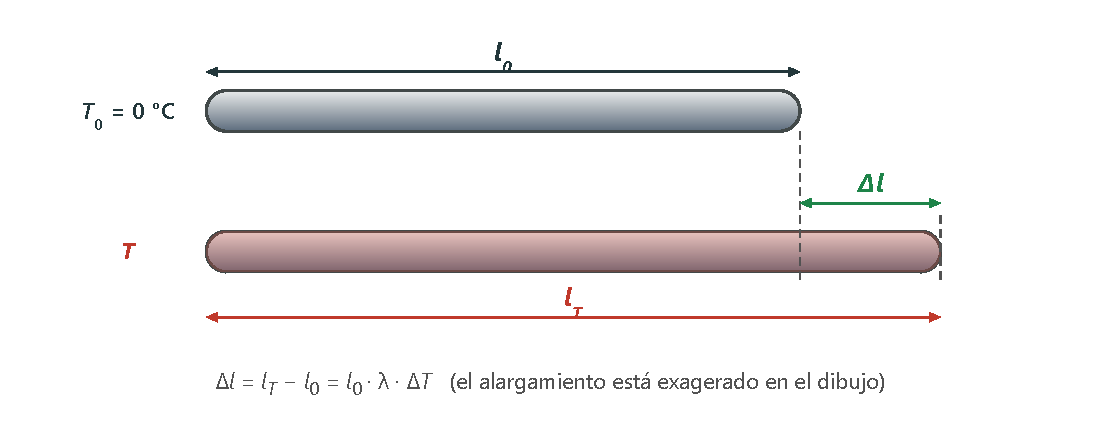
\includegraphics[width=0.85\textwidth]{images/UD12/dilatacion}
    \caption{Dilatación lineal de una barra al aumentar su temperatura.}
    \label{fig:dilatacion}
\end{figure}

\begin{definition}[Dilatación lineal]
    La \textbf{dilatación lineal} es el aumento de longitud que experimenta un cuerpo al calentarse. Si \(l_0\) es su longitud a \qty{0}{\degreeCelsius}, a la temperatura \(T\) (en \unit{\degreeCelsius}) su longitud es:
    \[ \boxed{l_T = l_0 \cdot (1 + \lambda \cdot T)} \qquad \Delta l = l_T - l_0 = l_0 \cdot \lambda \cdot T \]
    \(\lambda\) es el \textbf{coeficiente de dilatación lineal}: lo que se alarga cada metro de la sustancia, medido a \qty{0}{\degreeCelsius}, cuando su temperatura sube \qty{1}{\degreeCelsius}. Es característico de cada sustancia y se mide en \unit[per-mode=power]{\per\degreeCelsius}.
\end{definition}

En general, si la longitud inicial no está medida a \qty{0}{\degreeCelsius}, se usa la variación de temperatura: \(\Delta l = l_0 \cdot \lambda \cdot \Delta T\).

\begin{center}
    % --- tabla antigua ---
    % \begin{tblr}{colspec={lc}, hlines, vlines, row{1}={bg=ocre!85, fg=white, font=\bfseries}}
        % Sustancia & \(\lambda\) (\(\times 10^{-5}\) \unit[per-mode=power]{\per\degreeCelsius}) \\
        % Aluminio & \num{2.4} \\
        % Cobre & \num{1.8} \\
        % Hierro & \num{1.2} \\
        % Acero & \num{1.1} \\
        % Vidrio & \num{0.1}--\num{1.3} \\
        % Hormigón & \num{0.7}--\num{1.4} \\
    % \end{tblr}
    % --- tabla nueva ---
    \begin{tabular}{@{}lc@{}}
        \toprule
        \textbf{Sustancia} & \textbf{\(\lambda\) (\(\times 10^{-5}\) \unit[per-mode=power]{\per\degreeCelsius})} \\
        \midrule
        Aluminio & \num{2.4} \\[3pt]
        Cobre & \num{1.8} \\[3pt]
        Hierro & \num{1.2} \\[3pt]
        Acero & \num{1.1} \\[3pt]
        Vidrio & \num{0.1}--\num{1.3} \\[3pt]
        Hormigón & \num{0.7}--\num{1.4} \\
        \bottomrule
    \end{tabular}
\end{center}

\begin{example}
    Una barra de aluminio mide \qty{5}{\m} a \qty{0}{\degreeCelsius}. ¿Qué longitud tiene a \qty{40}{\degreeCelsius}? Dato: \(\lambda_{\text{Al}} = \qty[per-mode=power]{2.4e-5}{\per\degreeCelsius}\).
    \[ l_T = l_0 \cdot (1 + \lambda \cdot T) = 5 \cdot (1 + \num{2.4e-5} \cdot 40) = \textcolor{red}{\qty{5.0048}{\m}} \]
    La barra se ha alargado \qty{4.8}{\mm}: muy poco, pero suficiente para que haya que tenerlo en cuenta en las construcciones.
\end{example}

Los \textbf{líquidos} y los \textbf{gases} se dilatan mucho más que los sólidos. En ello se basan los termómetros de líquido: al calentarse, el mercurio o el alcohol se dilatan y suben por un tubo muy estrecho. El agua tiene un comportamiento anómalo: entre \qty{0}{\degreeCelsius} y \qty{4}{\degreeCelsius}, al calentarse se \emph{contrae}, y su densidad es máxima a \qty{4}{\degreeCelsius}. Por eso, en invierno, el fondo de los lagos se queda a unos \qty{4}{\degreeCelsius} y el hielo flota en la superficie, lo que permite que la vida acuática sobreviva.

\begin{exercise}
    Tenemos dos barras de hierro que, a \qty{0}{\degreeCelsius}, miden \qty{1.5}{\m} y \qty{3}{\m}. Calcula la longitud de la primera a \qty{80}{\degreeCelsius} y cuánto se alarga la segunda a \qty{150}{\degreeCelsius}. Dato: \(\lambda_{\text{Fe}} = \qty[per-mode=power]{1.2e-5}{\per\degreeCelsius}\).
    \begin{solu}
        \textcolor{blue}{Primera barra:} \(l_T = \num{1.5} \cdot (1 + \num{1.2e-5} \cdot 80) = \textcolor{red}{\qty{1.50144}{\m}}\).

        \textcolor{blue}{Segunda barra:} \(\Delta l = l_0 \cdot \lambda \cdot T = 3 \cdot \num{1.2e-5} \cdot 150 = \qty{5.4e-3}{\m} = \textcolor{red}{\qty{5.4}{\mm}}\).
    \end{solu}
\end{exercise}

\begin{exercise}
    Un raíl de acero mide \qty{25}{\m} a \qty{0}{\degreeCelsius}. ¿Cuánto se alarga en un día de verano en que se encuentra a \qty{45}{\degreeCelsius}? Dato: \(\lambda_{\text{acero}} = \qty[per-mode=power]{1.1e-5}{\per\degreeCelsius}\).
    \begin{solu}
        \(\Delta l = l_0 \cdot \lambda \cdot T = 25 \cdot \num{1.1e-5} \cdot 45 = \qty{0.0124}{\m} \approx \textcolor{red}{\qty{12.4}{\mm}}\); el raíl mide unos \qty{25.012}{\m}.
    \end{solu}
\end{exercise}

\begin{exercise}
    No conseguimos desenroscar la tapa metálica de un tarro de cristal. ¿Cómo podríamos lograrlo con agua caliente? Justifica tu respuesta.
    \begin{solu}
        Poniendo la tapa bajo un \textcolor{red}{chorro de agua caliente}. El metal tiene un coeficiente de dilatación mayor que el vidrio, así que la tapa \textcolor{red}{se dilata más que la boca del tarro}, queda más holgada y se puede desenroscar.
    \end{solu}
\end{exercise}

\subsection*{Actividades de consolidación: la dilatación}

\begin{exercise}
    Copia y completa: «El coeficiente de dilatación lineal del cobre es \qty[per-mode=power]{1.8e-5}{\per\degreeCelsius}. Esto quiere decir que \qty{1}{\m} de cobre, medido a \qty{0}{\degreeCelsius}, se alarga \ldots{} cuando su temperatura sube \qty{1}{\degreeCelsius}».
    \begin{solu}
        \ldots{} se alarga \textcolor{red}{\qty{1.8e-5}{\m}} (es decir, \qty{0.018}{\mm}).
    \end{solu}
\end{exercise}

\begin{exercise}
    Cuando se dilata una chapa metálica (dos dimensiones), ¿se trata de una dilatación lineal, superficial o cúbica?
    \begin{solu}
        De una dilatación \textcolor{red}{superficial}.
    \end{solu}
\end{exercise}

\begin{exercise}
    Algunos puentes son casi un metro más largos en verano que en invierno. Investiga qué se hace para que no se deformen.
    \begin{solu}
        Respuesta libre. Se construyen con \textcolor{red}{juntas de dilatación}: huecos entre tramos (a menudo cubiertos con piezas metálicas en forma de peine) que permiten que el tablero se alargue y se acorte sin deformarse. Además, el tablero se apoya sobre apoyos deslizantes o de neopreno.
    \end{solu}
\end{exercise}

\begin{exercise}
    Investiga qué efectos tiene la dilatación en las estructuras de hormigón y para qué sirven las juntas de dilatación.
    \begin{solu}
        Respuesta libre. Al calentarse y enfriarse, el hormigón se dilata y se contrae; si no tiene espacio, aparecen \textcolor{red}{tensiones que lo agrietan}. Las \textcolor{red}{juntas de dilatación} dividen la estructura en partes separadas por un pequeño hueco, de modo que cada parte puede dilatarse y contraerse libremente.
    \end{solu}
\end{exercise}

\begin{exercise}
    Investiga cómo afecta la dilatación a los raíles del tren y cómo se evitan sus efectos en la actualidad.
    \begin{solu}
        Respuesta libre. Si los raíles no pudieran alargarse, con el calor se \textcolor{red}{combarían} y el tren podría descarrilar. Antes se dejaba un pequeño \textcolor{red}{hueco entre raíles} (por eso sonaba el «traqueteo»). Hoy, en las líneas modernas, los raíles se sueldan en barras muy largas que se colocan \textcolor{red}{tensadas} y bien sujetas a las traviesas, para que no puedan dilatarse, y se usan aparatos de dilatación en algunos puntos.
    \end{solu}
\end{exercise}

\begin{exercise}
    La figura muestra la lámina bimetálica de un termostato: dos láminas de metales con distinto coeficiente de dilatación, soldadas entre sí. Explica cómo funciona.
    \begin{center}
        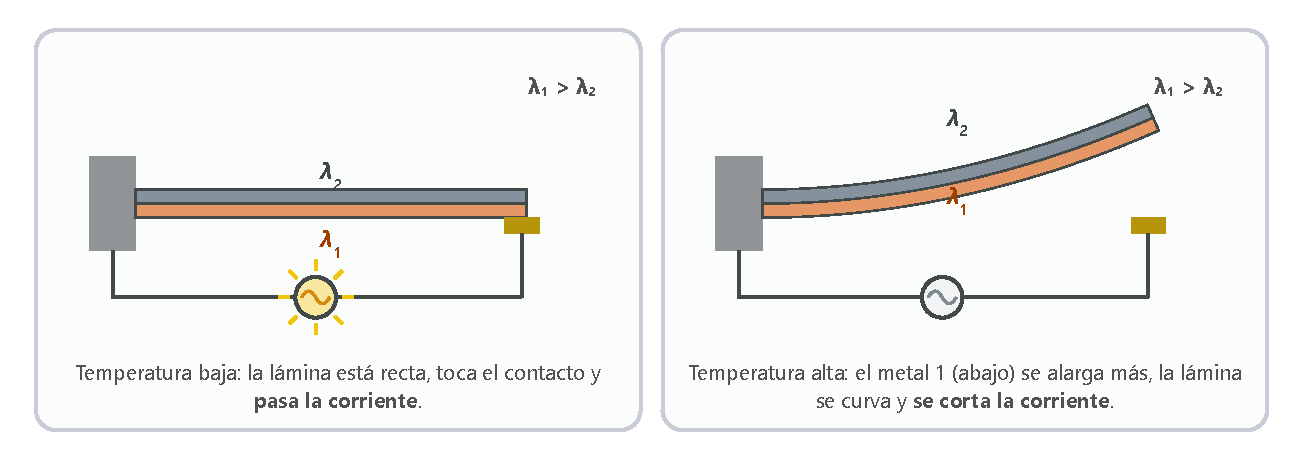
\includegraphics[width=0.9\textwidth]{images/UD12/bimetal}
    \end{center}
    \begin{solu}
        Al subir la temperatura, el metal de mayor coeficiente de dilatación (\(\lambda_1\)) se alarga más que el otro. Como están soldados, la lámina \textcolor{red}{se curva}, quedando el metal que más se dilata en la parte exterior (convexa). Al curvarse, la lámina \textcolor{red}{se separa del contacto y corta la corriente} (por ejemplo, la de la resistencia de una plancha o de un radiador). Cuando se enfría, vuelve a estar recta, cierra el circuito y la corriente pasa de nuevo. Así se mantiene la temperatura alrededor de un valor.
    \end{solu}
\end{exercise}

\begin{exercise}
    Usando la tabla de coeficientes de dilatación lineal, calcula cuánto se alarga \qty{1}{\m} de cada material cuando su temperatura sube de \qty{0}{\degreeCelsius} a \qty{40}{\degreeCelsius}.
    \begin{solu}
        \(\Delta l = l_0 \cdot \lambda \cdot T = 1 \cdot \lambda \cdot 40\):
        \begin{center}
            % --- tabla antigua ---
            % \begin{tblr}{colspec={lc}, hlines, vlines, row{1}={bg=ocre!85, fg=white, font=\bfseries}}
                % Material & \(\Delta l\) (m) \\
                % Aluminio & \num{9.6e-4} \\
                % Cobre & \num{7.2e-4} \\
                % Hierro & \num{4.8e-4} \\
                % Acero & \num{4.4e-4} \\
                % Vidrio & entre \num{4e-5} y \num{5.2e-4} \\
                % Hormigón & entre \num{2.8e-4} y \num{5.6e-4} \\
            % \end{tblr}
            % --- tabla nueva ---
            \begin{tabular}{@{}lc@{}}
                \toprule
                \textbf{Material} & \textbf{\(\Delta l\) (m)} \\
                \midrule
                Aluminio & \num{9.6e-4} \\[3pt]
                Cobre & \num{7.2e-4} \\[3pt]
                Hierro & \num{4.8e-4} \\[3pt]
                Acero & \num{4.4e-4} \\[3pt]
                Vidrio & entre \num{4e-5} y \num{5.2e-4} \\[3pt]
                Hormigón & entre \num{2.8e-4} y \num{5.6e-4} \\
                \bottomrule
            \end{tabular}
        \end{center}
    \end{solu}
\end{exercise}

%========================================================================================
\section{Equivalencia entre energía mecánica y energía térmica}
%========================================================================================

Sabemos que la combustión no es la única forma de producir energía térmica: también se obtiene a partir de la energía mecánica. Basta con frotarse las manos, frenar una bicicleta o taladrar una pieza de metal, como observó Thompson.

\subsection{¿Qué relación cuantitativa existe entre el trabajo y el calor?}

En 1845, el físico inglés \textbf{James Prescott Joule} demostró experimentalmente que el trabajo y el calor son equivalentes. En su experimento más famoso (figura~\ref{fig:joule}), unas pesas caían desde cierta altura y, al bajar, hacían girar unas paletas dentro de un recipiente con agua, aislado del exterior. El rozamiento de las paletas con el agua aumentaba su temperatura. Joule midió la energía potencial que perdían las pesas y el calor que ganaba el agua, y comprobó que, \textbf{siempre que se realiza la misma cantidad de trabajo, se obtiene la misma cantidad de calor}, tanto si el trabajo es mecánico como si es eléctrico o químico.

\begin{figure}[H]
    \centering
    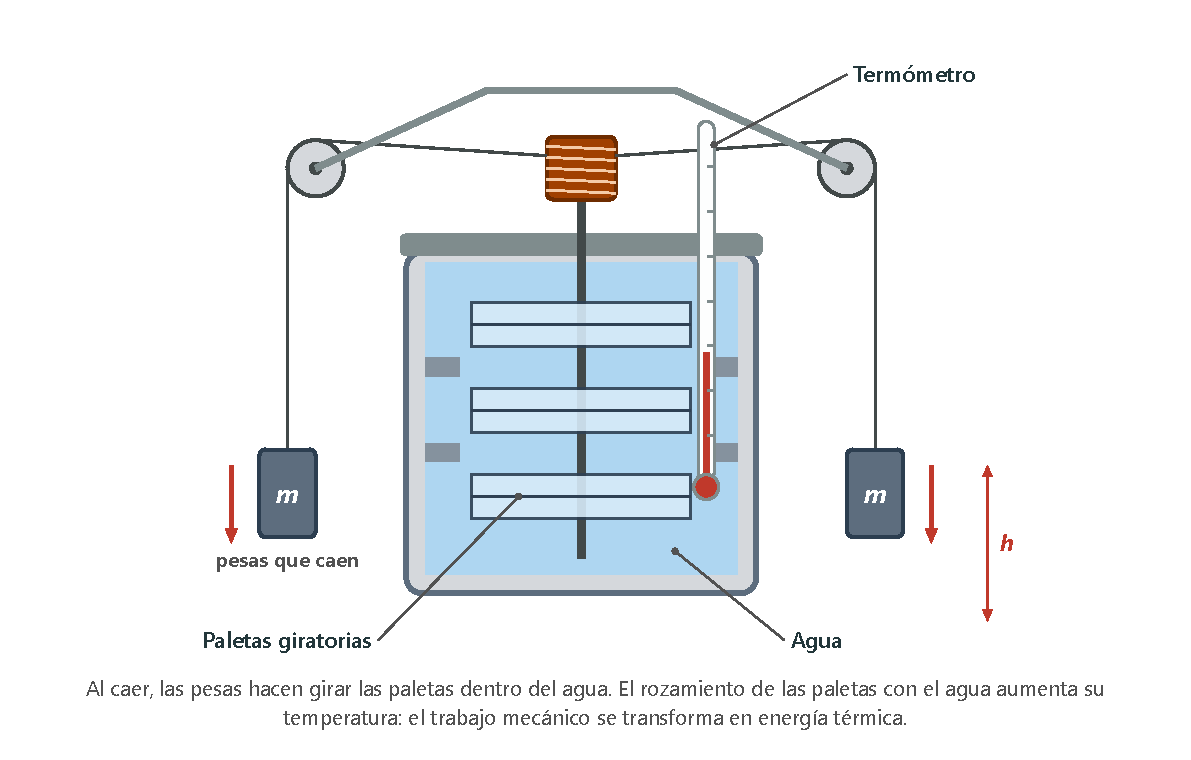
\includegraphics[width=0.85\textwidth]{images/UD12/joule}
    \caption{Experimento de Joule para demostrar la equivalencia entre trabajo y calor.}
    \label{fig:joule}
\end{figure}

\begin{definition}[Equivalente mecánico del calor]
    Si el trabajo y el calor se miden en las mismas unidades, la relación encontrada por Joule es simplemente:
    \[ W = Q \]
    Este resultado se conoce como \textbf{equivalente mecánico del calor}. Cuando el calor se medía en calorías, Joule encontró que \(\qty{1}{\calorie} = \qty{4.18}{\joule}\).
\end{definition}

El resultado de Joule es otra forma de expresar el \textbf{principio de conservación de la energía}, ahora incluyendo el calor como forma de transferir energía:

\begin{marker}
    La \textbf{energía total} de un sistema aislado permanece \textbf{constante}: la energía no se crea ni se destruye, solo se transforma o se transfiere (mediante trabajo o calor).
\end{marker}

\begin{example}
    En una cascada de \qty{50}{\m} de altura, ¿cuánto aumentaría la temperatura del agua si toda su energía potencial se transformase en energía térmica del agua al chocar abajo? (Joule intentó medirlo durante su luna de miel en Suiza.)

    Para una masa \(m\) de agua, igualamos la energía potencial perdida con el calor que gana:
    \[ m \cdot g \cdot h = m \cdot c \cdot \Delta T \Rightarrow \Delta T = \frac{g \cdot h}{c} = \frac{\num{9.8} \cdot 50}{4180} = \textcolor{red}{\qty{0.12}{\degreeCelsius}} \]
    La masa se simplifica. El aumento es muy pequeño: hace falta mucho trabajo para calentar el agua.
\end{example}

\subsection{La degradación de la energía}

\begin{marker}
    Es fácil transformar \textbf{toda} la energía mecánica en energía térmica, pero \textbf{no es posible transformar totalmente la energía térmica en energía mecánica}.
\end{marker}

Por ejemplo, el trabajo de las fuerzas de rozamiento se convierte por completo en calor. En cambio, una máquina térmica solo consigue aprovechar como trabajo una parte de la energía térmica que recibe; el resto se transfiere al ambiente. Por eso decimos que la energía se \textbf{degrada}: en cada transformación, aunque la cantidad total se conserva, una parte acaba en una forma \textbf{menos útil para realizar trabajo} (energía térmica repartida por el ambiente a baja temperatura). La energía útil siempre es menor que la energía total.

\begin{definition}[Rendimiento]
    El \textbf{rendimiento} de cualquier transformación de energía es el porcentaje de la energía total que se aprovecha:
    \[ \text{rendimiento} = \frac{\text{energía útil}}{\text{energía total}} \cdot 100 \]
\end{definition}

\begin{example}
    A una máquina se le suministran \qty{400}{\joule}, de los cuales solo aprovecha \qty{100}{\joule} como trabajo. ¿Cuál es su rendimiento?
    \[ \text{rendimiento} = \frac{100}{400} \cdot 100 = \textcolor{red}{\qty{25}{\percent}} \]
    Los \qty{300}{\joule} restantes no desaparecen: se transfieren al ambiente, sobre todo como calor.
\end{example}

\begin{exercise}
    Frota con fuerza una lima de hierro contra una superficie metálica durante unos minutos. ¿Qué les ocurre a la lima y a la superficie? ¿Qué transformación de energía se ha producido?
    \begin{solu}
        Las dos \textcolor{red}{se calientan}: el trabajo de las fuerzas de rozamiento se ha transformado en \textcolor{red}{energía térmica}.
    \end{solu}
\end{exercise}

\begin{exercise}
    ¿Puede ser del \qty{100}{\percent} el rendimiento de una máquina que transforma energía térmica en mecánica? ¿Por qué?
    \begin{solu}
        \textcolor{red}{No}. La energía térmica no puede transformarse por completo en energía mecánica: siempre se transfiere una parte al ambiente como calor, así que el rendimiento de una máquina térmica es siempre \textcolor{red}{menor del \qty{100}{\percent}}.
    \end{solu}
\end{exercise}

\subsection*{Actividades de consolidación: equivalencia entre trabajo y calor}

\begin{exercise}
    ¿Qué se conoce como equivalente mecánico del calor? ¿Quién lo determinó?
    \begin{solu}
        Es la equivalencia entre trabajo y calor: una misma cantidad de trabajo produce siempre la misma cantidad de calor. Si los dos se miden en julios, \textcolor{red}{\(W = Q\)}; con la antigua unidad de calor, \(\qty{1}{\calorie} = \qty{4.18}{\joule}\). Lo determinó \textcolor{red}{James Prescott Joule} en 1845.
    \end{solu}
\end{exercise}

\begin{exercise}
    Dobla un alambre fino varias veces por el mismo sitio. Comprueba que se calienta en esa zona e identifica la transformación de energía que se produce. ¿Puede realizarse la transformación inversa por completo?
    \begin{solu}
        Se transforma \textcolor{red}{energía mecánica (trabajo) en energía térmica}. La transformación inversa \textcolor{red}{no puede realizarse por completo}: no es posible convertir toda la energía térmica en trabajo.
    \end{solu}
\end{exercise}

\begin{exercise}
    ¿Cuál es el rendimiento de una transformación energética si de \qty{8e6}{\joule} solo se aprovechan \qty{5.2e6}{\joule}?
    \begin{solu}
        \(\text{rendimiento} = \dfrac{\num{5.2e6}}{\num{8e6}} \cdot 100 = \textcolor{red}{\qty{65}{\percent}}\).
    \end{solu}
\end{exercise}

\begin{exercise}
    Los procesos que cumplen el principio de conservación de la energía pero nunca ocurren espontáneamente al revés se llaman \textbf{irreversibles}.
    \begin{enumerate}[label=\alph*)]
        \item Al poner en contacto dos cuerpos a diferente temperatura, el caliente cede energía al frío hasta que alcanzan el equilibrio térmico. ¿Puede ocurrir espontáneamente el proceso inverso? ¿Es irreversible?
        \item Al abrir un frasco de perfume, este se evapora y se reparte por la habitación. ¿Puede ocurrir espontáneamente el proceso inverso? ¿Es irreversible?
    \end{enumerate}
    \begin{solu}
        a) \textcolor{red}{No}: nunca se ha visto que dos cuerpos a la misma temperatura se separen espontáneamente en uno caliente y otro frío. Es un \textcolor{red}{proceso irreversible}.
        b) \textcolor{red}{No}: el perfume repartido por la habitación no vuelve solo al frasco. También es \textcolor{red}{irreversible}.
    \end{solu}
\end{exercise}

\begin{exercise}
    ¿Qué significa que el rendimiento de una transformación energética es del \qty{50}{\percent}?
    \begin{solu}
        Que solo se aprovecha como energía útil \textcolor{red}{la mitad} de la energía total suministrada; la otra mitad se transfiere al ambiente, sobre todo como calor.
    \end{solu}
\end{exercise}

\begin{exercise}
    Un coche de \qty{1200}{\kg} que circula a \qty{72}{\km\per\hour} frena hasta pararse. ¿Cuánta energía cinética se transforma en energía térmica en los frenos? Si toda esa energía calentara los discos de freno (\qty{8}{\kg} de acero en total, \(c = \qty{450}{\cunit}\)), ¿cuánto subiría su temperatura?
    \begin{solu}
        \(v = \qty{72}{\km\per\hour} = \qty{20}{\m\per\s}\). \(E_c = \frac{1}{2} \cdot 1200 \cdot 20^2 = \textcolor{red}{\qty{240000}{\joule}}\).

        \(\Delta T = \dfrac{Q}{m \cdot c} = \dfrac{\num{240000}}{8 \cdot 450} \approx \textcolor{red}{\qty{67}{\degreeCelsius}}\). Por eso los frenos se calientan tanto en una bajada larga.
    \end{solu}
\end{exercise}

%========================================================================================
\section[Las máquinas térmicas]{Aplicaciones de la transformación de energía térmica en energía mecánica: las máquinas térmicas}
%========================================================================================

Una \textbf{máquina térmica} es un dispositivo que transforma en energía mecánica (trabajo) parte del calor obtenido, normalmente, de la combustión de un combustible. Toda máquina térmica funciona entre un \textbf{foco caliente} (la caldera o la cámara de combustión) y un \textbf{foco frío} (el condensador, el refrigerante o el propio ambiente).

\begin{figure}[H]
    \centering
    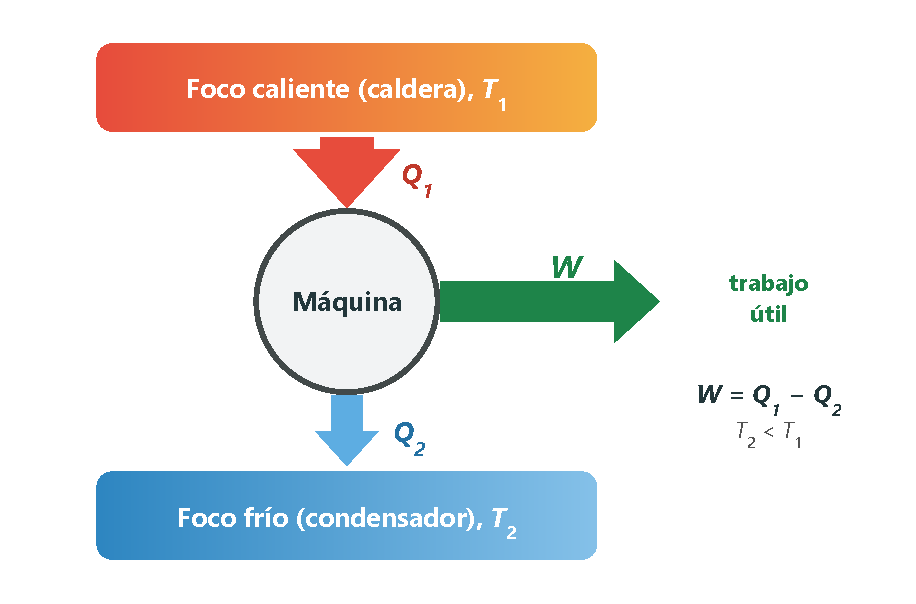
\includegraphics[width=0.7\textwidth]{images/UD12/maquina_termica}
    \caption{Esquema de funcionamiento de una máquina térmica.}
    \label{fig:maquina_termica}
\end{figure}

Como muestra la figura~\ref{fig:maquina_termica}, la máquina toma un calor \(Q_1\) del foco caliente, que está a la temperatura \(T_1\); convierte una parte en trabajo mecánico, \(W\), y cede el resto, \(Q_2\), al foco frío, que está a una temperatura menor, \(T_2\). La energía útil es:
\[ W = Q_1 - Q_2 \]

El rendimiento de la máquina térmica, \(R\), es:
\[ R = \frac{W}{Q_1} \cdot 100 = \frac{Q_1 - Q_2}{Q_1} \cdot 100 \]

El rendimiento \textbf{máximo} (teórico) que puede alcanzar una máquina térmica depende solo de las temperaturas absolutas (en kelvin) del foco caliente, \(T_1\), y del foco frío, \(T_2\):
\[ \boxed{R_{\text{máx}} = \frac{T_1 - T_2}{T_1} \cdot 100} \]
Las máquinas reales tienen siempre un rendimiento menor que este, por los rozamientos y las pérdidas de calor. Cuanto mayor es la diferencia de temperatura entre los focos, mayor es el rendimiento posible.

Según dónde se queme el combustible, las máquinas térmicas son:
\begin{itemize}
    \item De \textbf{combustión externa}: el combustible se quema fuera de la máquina, por ejemplo, en una caldera (máquina de vapor, turbina de vapor).
    \item De \textbf{combustión interna}: el combustible se quema dentro del motor (motores de gasolina y diésel, turbinas de los aviones).
\end{itemize}

\begin{example}
    Una máquina térmica recibe \qty{5000}{\joule} del foco caliente y realiza un trabajo de \qty{1500}{\joule}. ¿Cuál es su rendimiento? ¿Cuánto calor cede al foco frío?
    \[ R = \frac{W}{Q_1} \cdot 100 = \frac{1500}{5000} \cdot 100 = \textcolor{red}{\qty{30}{\percent}} \qquad Q_2 = Q_1 - W = 5000 - 1500 = \textcolor{red}{\qty{3500}{\joule}} \]
\end{example}

\subsection{La máquina de vapor}

La \textbf{máquina de vapor} es una máquina de combustión externa (figura~\ref{fig:maquina_vapor}). En una caldera se calienta agua a alta presión hasta que se convierte en vapor a muy alta temperatura. El vapor pasa al cilindro, se expande y empuja el pistón, que realiza un trabajo: mediante una biela, el movimiento de vaivén del pistón se convierte en el giro de un volante. Después, el vapor, ya más frío, pasa al condensador, donde vuelve a ser agua líquida, y una bomba la devuelve a la caldera para empezar de nuevo.

\begin{figure}[H]
    \centering
    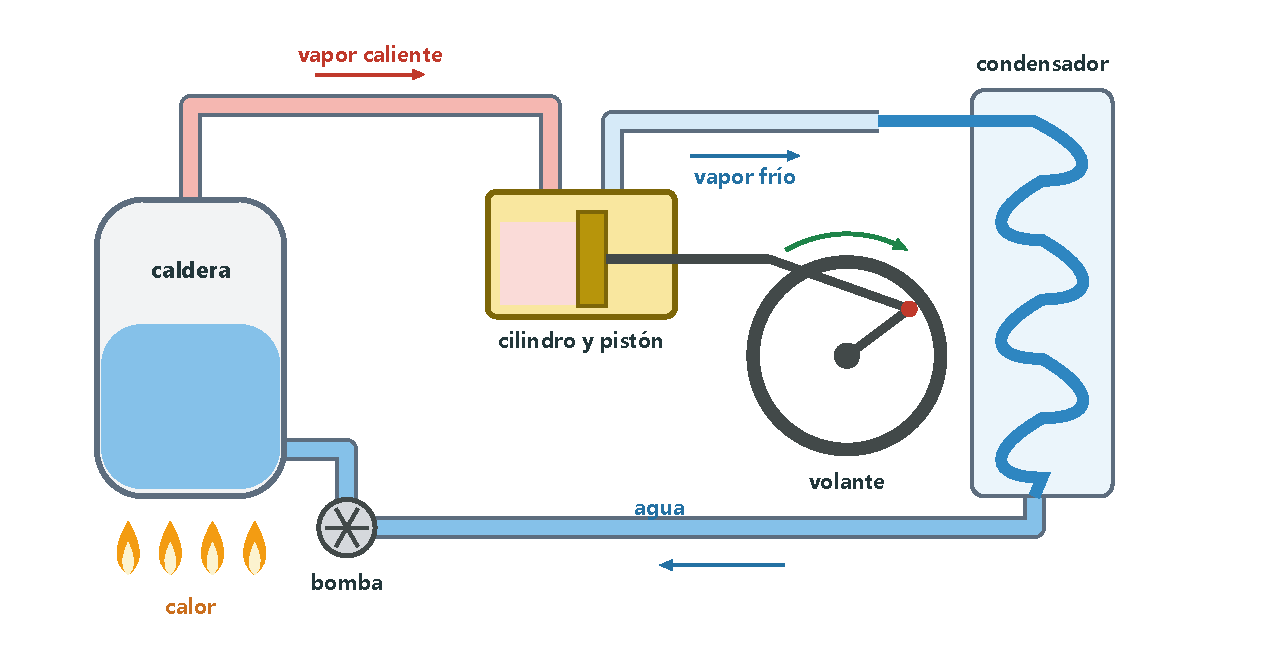
\includegraphics[width=\textwidth]{images/UD12/maquina_vapor}
    \caption{Esquema de una máquina de vapor.}
    \label{fig:maquina_vapor}
\end{figure}

La máquina de vapor, perfeccionada por James Watt a finales del siglo \textsc{xviii}, impulsó la Revolución Industrial: movió fábricas, locomotoras y barcos. Hoy se utilizan \textbf{turbinas de vapor}, que funcionan con el mismo principio en las centrales térmicas y nucleares.

\begin{example}
    Calcula el rendimiento máximo de una máquina de vapor en la que el vapor entra en el cilindro a \qty{220}{\degreeCelsius} y sale a \qty{100}{\degreeCelsius}.

    Pasamos las temperaturas a kelvin: \(T_1 = 220 + 273 = \qty{493}{\kelvin}\); \(T_2 = 100 + 273 = \qty{373}{\kelvin}\).
    \[ R = \frac{T_1 - T_2}{T_1} \cdot 100 = \frac{493 - 373}{493} \cdot 100 = \textcolor{red}{\qty{24.3}{\percent}} \]
    Incluso en el caso ideal, más de las tres cuartas partes de la energía se pierden.
\end{example}

\begin{exercise}
    Calcula el rendimiento máximo de una máquina de vapor en la que el vapor entra en el cilindro a \qty{260}{\degreeCelsius} y sale a \qty{120}{\degreeCelsius}.
    \begin{solu}
        \(T_1 = 260 + 273 = \qty{533}{\kelvin}\); \(T_2 = 120 + 273 = \qty{393}{\kelvin}\).
        \[ R = \frac{533 - 393}{533} \cdot 100 = \textcolor{red}{\qty{26.3}{\percent}} \]
    \end{solu}
\end{exercise}

\begin{exercise}
    Las máquinas de vapor de pistón han sido sustituidas por las turbinas de vapor. Busca información sobre cómo funcionan y qué ventajas tienen.
    \begin{solu}
        Respuesta libre. En una \textcolor{red}{turbina de vapor}, el vapor que sale de la caldera a gran presión pasa por unas coronas de paletas fijas, que lo dirigen, y empuja las paletas de unas ruedas móviles, que giran unidas a un eje. Ventajas: el \textcolor{red}{giro se obtiene directamente} (sin pistón ni biela), alcanzan \textcolor{red}{gran velocidad y potencia}, funcionan de forma continua, con menos vibraciones, y tienen mejor rendimiento. Se usan en las centrales eléctricas para mover los alternadores.
    \end{solu}
\end{exercise}

\subsection{El motor de combustión interna}

¿Todas las máquinas térmicas tienen caldera? No: en el \textbf{motor de combustión interna}, el combustible se quema dentro del propio cilindro. Además, la mezcla de aire y combustible se comprime antes de quemarse, lo que aumenta el rendimiento y reduce el consumo.

El más conocido es el \textbf{motor de explosión de cuatro tiempos}, que usa gasolina. Cada cilindro tiene dos orificios cerrados por válvulas: la de \textbf{admisión}, por la que entra la mezcla, y la de \textbf{escape}, por la que salen los gases quemados. En la parte superior hay una \textbf{bujía}, que produce la chispa que inicia la combustión. El pistón (o émbolo) está unido por una biela al \textbf{cigüeñal}, que transforma el movimiento de subida y bajada en giro. El motor repite cíclicamente cuatro fases o tiempos; en cada una, el pistón recorre el cilindro una vez (una carrera) y el cigüeñal da media vuelta (figura~\ref{fig:motor_cuatro_tiempos}).

\begin{figure}[H]
    \centering
    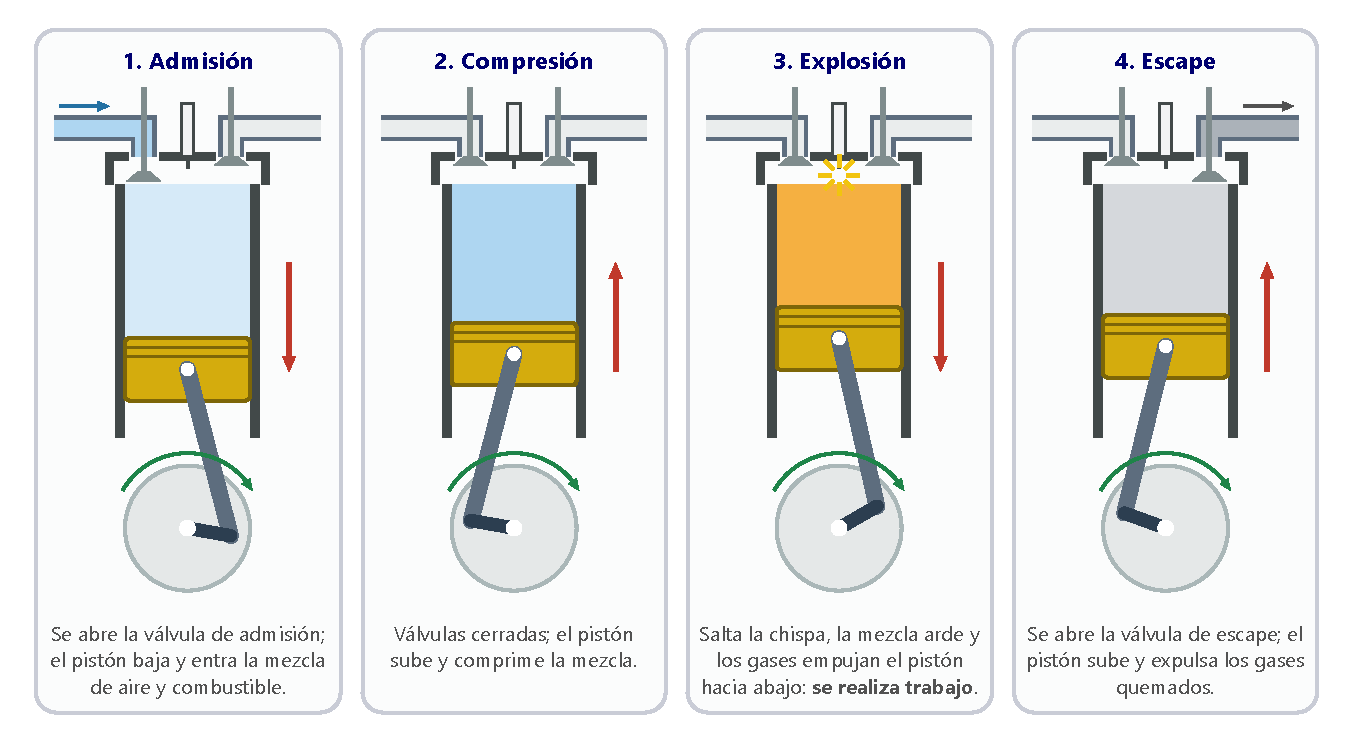
\includegraphics[width=\textwidth]{images/UD12/motor_cuatro_tiempos}
    \caption{Los cuatro tiempos de un motor de explosión.}
    \label{fig:motor_cuatro_tiempos}
\end{figure}

\begin{enumerate}[label=\numberballblue]
    \item \textbf{Admisión}. La válvula de admisión está abierta y la de escape, cerrada. El pistón baja y entra en el cilindro la mezcla de aire y gasolina. El cigüeñal gira media vuelta.
    \item \textbf{Compresión}. Las dos válvulas se cierran. El pistón sube y comprime la mezcla, que se calienta. El cigüeñal gira otra media vuelta.
    \item \textbf{Explosión} (o expansión). Con las válvulas cerradas, salta la chispa de la bujía y la mezcla se quema muy deprisa. Los gases calientes que se producen aumentan bruscamente la presión y empujan el pistón hacia abajo: es el único tiempo en el que \textbf{se realiza trabajo}. El cigüeñal gira otra media vuelta.
    \item \textbf{Escape}. Se abre la válvula de escape, el pistón sube y expulsa al exterior los gases de la combustión (sobre todo \ch{CO2} y vapor de agua). El cigüeñal gira otra media vuelta y, en total, ha dado dos vueltas completas. El ciclo vuelve a empezar.
\end{enumerate}

Los motores \textbf{diésel} también son de cuatro tiempos, pero no tienen bujía: el aire se comprime tanto que se calienta por encima de la temperatura de ignición del gasóleo, que se inyecta y arde solo.

\begin{exercise}
    ¿En cuál de los cuatro tiempos de un motor de explosión se realiza trabajo?
    \begin{solu}
        En el \textcolor{red}{tercer tiempo, la explosión}: los gases de la combustión empujan el pistón hacia abajo. En los otros tres tiempos el cigüeñal sigue girando gracias a la inercia del volante (y a los demás cilindros del motor).
    \end{solu}
\end{exercise}

\begin{exercise}
    ¿Cuántas vueltas completas da el cigüeñal durante los cuatro tiempos de un motor de explosión?
    \begin{solu}
        Media vuelta en cada tiempo: en total, \textcolor{red}{dos vueltas completas}.
    \end{solu}
\end{exercise}

\subsection*{Actividades de consolidación: las máquinas térmicas}

\begin{exercise}
    Relaciona cada tiempo del motor de combustión interna (admisión, compresión, explosión, escape) con su descripción:
    \begin{enumerate}[label=\Alph*.]
        \item Al quemarse el combustible, los gases se expanden y empujan el pistón hacia abajo.
        \item El pistón baja y permite la entrada de la mezcla de gasolina y aire.
        \item El pistón sube y empuja los gases fuera del cilindro.
        \item El pistón sube y comprime la mezcla antes de la chispa.
    \end{enumerate}
    \begin{solu}
        \textcolor{red}{Admisión: B; compresión: D; explosión: A; escape: C}.
    \end{solu}
\end{exercise}

\begin{exercise}
    ¿Qué es una máquina térmica? ¿Cuál es el rendimiento de una máquina térmica que recibe \qty{8e6}{\joule} del foco caliente y realiza un trabajo de \qty{2.8e6}{\joule}? ¿Qué calor cede al foco frío?
    \begin{solu}
        Es un dispositivo que \textcolor{red}{transforma en trabajo mecánico parte del calor} que recibe de un foco caliente, cediendo el resto a un foco frío.
        \(R = \dfrac{\num{2.8e6}}{\num{8e6}} \cdot 100 = \textcolor{red}{\qty{35}{\percent}}\); \(Q_2 = Q_1 - W = \textcolor{red}{\qty{5.2e6}{\joule}}\).
    \end{solu}
\end{exercise}

\begin{exercise}
    Calcula el rendimiento máximo de una máquina de vapor en la que el vapor entra en el cilindro a \qty{190}{\degreeCelsius} y sale a \qty{90}{\degreeCelsius}.
    \begin{solu}
        \(T_1 = \qty{463}{\kelvin}\); \(T_2 = \qty{363}{\kelvin}\). \(R = \dfrac{463 - 363}{463} \cdot 100 = \textcolor{red}{\qty{21.6}{\percent}}\).
    \end{solu}
\end{exercise}

\begin{exercise}
    ¿Por qué no se pueden usar las temperaturas en grados Celsius en la fórmula \(R = \dfrac{T_1 - T_2}{T_1} \cdot 100\)? Compruébalo con los datos de la actividad anterior.
    \begin{solu}
        Porque el numerador es una diferencia (vale lo mismo en \unit{\degreeCelsius} que en \unit{\kelvin}), pero el denominador no: hay que usar la \textcolor{red}{temperatura absoluta}. Con grados Celsius saldría \(\frac{190 - 90}{190} \cdot 100 = \qty{52.6}{\percent}\), un valor \textcolor{red}{erróneo}, mucho mayor que el real (\qty{21.6}{\percent}).
    \end{solu}
\end{exercise}
